% Thesis revision, begun 9 October 2026; professor feedback incorporated 2 November 2026.
% Retained performance evidence: MSD/ADNI four-model capped studies (504 each),
% MSD MedSAM3: one campaign, 14 objectives, two execution batches (27 and 108 records); ADNI MedSAM3 (126).
% See reports/thesis_noaug_update_20261021/ for audited extraction and provenance.
% GeoFWI3D: 504 fixed fold/seed/objective cells integrated 22 October 2026.
% Geological UNETR uses XY D4 transformations in baseline and constrained arms.
% Geological cap includes calibration; see reports/thesis_geofwi_update_20261022/.
% SAM3: all 126 final runs verified and integrated 23 October 2026.
% Scores, fold effects, FN/FP and complementary Dice: reports/thesis_sam3_final_20261023/.
% Earlier structure and progress reports remain dated provenance snapshots.
% Background/all-class Dice integrated 23 October 2026 from verified evaluation archives.
% See reports/thesis_background_dice_update_20261023/ for numeric checks and patch.
% Existing dataset illustrations and annotation-compatibility audit are retained.
% Verified qualitative reproductions integrated 3 November 2026; original aggregates unchanged.
% Provenance: reports/thesis_qualitative_predictions_20261103/final_verification.json.
% Bibliography is embedded; figure assets are in figures/compiled and figures/qualitative.
% For Overleaf, upload thesis-revision.tex AND the complete figures folder together.

\documentclass[12pt,a4paper]{article}
\usepackage[T1]{fontenc}
\usepackage[utf8]{inputenc}
\usepackage[english]{babel}
\usepackage{lmodern}
\usepackage[a4paper,margin=2.5cm]{geometry}
\usepackage{amsmath,amssymb}
\usepackage{setspace,microtype}
\usepackage[hidelinks]{hyperref}
\usepackage{xurl}
\usepackage{graphicx}
\usepackage{tikz} % Only the compact, editable adaptation workflow is drawn live.
\usepackage[section]{placeins}
% Keep pending figures and tables inside the section that introduces them.
\AddToHook{cmd/subsection/before}{\FloatBarrier}
\AddToHook{cmd/subsubsection/before}{\FloatBarrier}
% Allow substantial figures alongside text without deferring them unnecessarily.
\renewcommand{\topfraction}{0.9}
\renewcommand{\bottomfraction}{0.8}
\renewcommand{\textfraction}{0.1}
\renewcommand{\floatpagefraction}{0.75}
\AddToHook{env/figure/begin}{\setstretch{1.05}}
% If a full figure page is needed, align its contents at the top.
\makeatletter
\setlength{\@fptop}{0pt}
\makeatother
\usepackage{array,longtable}
\newcolumntype{P}[1]{>{\raggedright\arraybackslash}p{#1}}
% Heavy figures are stored in figures/compiled; upload this folder with the TeX source.
\definecolor{thesisBlue}{RGB}{36,105,155}
\definecolor{thesisOrange}{RGB}{205,117,42}
\definecolor{thesisInk}{RGB}{39,49,60}
\definecolor{thesisGray}{RGB}{109,119,130}
\definecolor{thesisPaleBlue}{RGB}{235,243,249}
\definecolor{thesisPaleOrange}{RGB}{252,242,232}
\definecolor{thesisPaleGray}{RGB}{245,247,249}
% Numerical results are complete; evidence limitations are stated in Results.
\setstretch{1.3}
\setlength{\emergencystretch}{2em}
\raggedbottom


% Numerical tables generated from reports/thesis_noaug_update_20261021/results.json.
% Medical aggregates exclude augmented and historical epoch-policy/pilot results.
% Geological tables use the separately frozen final 504-cell campaign.

\begin{document}

% Submission version: abstract retained here, excluded from the compiled thesis.
% Set \thesisincludeabstracttrue if the programme requires it in the PDF.
\newif\ifthesisincludeabstract
\thesisincludeabstractfalse
\ifthesisincludeabstract
\section*{Abstract}

Semantic segmentation assigns a class to each location in an image,
turning measurements into structures that can be identified and measured.
In medical imaging, it supports quantitative analysis of organs and
anatomical regions, but learning accurate segmentations can require
substantial annotation and computation. This thesis investigates whether
spatial information in existing annotations can improve three-dimensional
segmentation when both resources are limited.

The approach uses Logic Tensor Networks (LTNs), a neuro-symbolic framework
that connects logical statements with differentiable learning, and their
logarithmic formulation, logLTN. Additional training objectives encourage
predictions to agree with annotated boundaries, neighbouring labels and
region geometry. The method is evaluated first on synthetic geological
volumes from GeoFWI3D and then on hippocampus magnetic resonance imaging
from the Medical Segmentation Decathlon (MSD) and Alzheimer's Disease
Neuroimaging Initiative (ADNI). Hippocampus delineation supports studies
of brain structure in a region affected by Alzheimer's disease.

Experiments cover both training from scratch and adapting pretrained
models, which start with representations learned from other images.
Across four architectures trained from scratch, the highest-mean tested
configurations improve Dice, a measure of region overlap, over matched
baselines by 1.16--6.14 percentage
points on GeoFWI3D, 5.35--11.97 points on MSD and 1.03--5.54 points on
ADNI. Adaptation of Segment Anything Model~3 (SAM3) reaches 72.76\% Dice
on GeoFWI3D, a gain of 3.45 points. Its medical specialization, MedSAM3,
reaches 81.73\% on MSD and 80.85\% on ADNI, with gains of 5.38 and
3.53 points. The preferred objective varies with the model and task.
The findings show that explicit spatial supervision can improve the
segmentation accuracy attainable from limited annotations and training,
including when adapting a pretrained model.

\clearpage
\fi
\setcounter{tocdepth}{2}
\tableofcontents
\clearpage
\section{Introduction}\label{sec:introduction}
\label{sec:motivation}\label{sec:research-questions}

Three-dimensional semantic segmentation identifies structures in an image
by assigning a class to every voxel, the three-dimensional counterpart
of a pixel. A stack of medical image slices can thereby become a map of
an organ; a geological image can become a map of a subsurface formation.
These maps make it possible to measure the size of a structure and study
its shape and relationship to its surroundings. Segmentation thus connects
image acquisition with quantitative analysis.

Traditionally, reference segmentations have been produced by delineating
structures in the images. A segmentation mask stores these decisions as
class labels on the image grid. In supervised learning, a neural network
learns to reproduce such masks from paired images and annotations.
Models such as U-Net and its three-dimensional extension learn image
features and use them to predict a mask, making this approach widely
applicable to biomedical images \cite{ronneberger2015unet,cicek2016unet}.
Transformer-based models learn how strongly information from different
image regions should influence a prediction. Pretrained models begin
with features learned from other images and can be adapted to a new task. These developments provide several routes to automatic
segmentation, but they do not remove two practical constraints:
\begin{itemize}
\item \textbf{Limited annotations.} Delineating a structure throughout a
volume takes time and can require specialist knowledge. In medical
imaging, uncertain boundaries further complicate consistent labelling
\cite{wang2021annotation}.
\item \textbf{Limited computation.} Training a volumetric model can be
expensive. An approach that reaches useful accuracy sooner may be
valuable even when a longer training run would eventually close the gap.
\end{itemize}

This thesis asks whether the spatial information already contained in a mask
can make learning more effective under these restrictions. Consider a voxel
just inside an annotated object: its label specifies membership, but its
location also tells us that it lies close to the object's edge. Two
neighbouring voxels reveal whether the annotation changes class at that
location. The proposed approach gives these relationships an explicit role
in the training objective, alongside the model's usual segmentation loss,
the numerical penalty for disagreement with the annotation. Training with
this usual loss alone provides the baseline against which the added
supervision is compared. No additional manual annotations are needed.

Logic Tensor Networks (LTNs) provide a way to express such supervision
\cite{badreddine2022logic}. They belong to neuro-symbolic artificial
intelligence, which combines neural learning with explicitly stated
knowledge. In an LTN, a statement such as ``these annotated inner voxels
belong to the object'' receives a numerical degree of satisfaction from the
model's predictions. Training can then increase that satisfaction. The
logarithmic formulation, logLTN, expresses these satisfaction values, also
called truth degrees, through their logarithms: multiplying degrees of
satisfaction becomes addition, and their negative logarithms give penalties
to minimize \cite{badreddine2023logltn}. Here, \emph{spatial constraints}
means soft training objectives: they encourage the stated properties without
guaranteeing them in every predicted segmentation.

Four forms of supervision are studied. The first reinforces membership
on either side of an annotated boundary. The second encourages
neighbouring predictions to reproduce the class transitions in the mask.
The third uses distance from each class boundary to weight membership
errors. The fourth balances class supervision across spatial layers of
the annotated region. The thesis connects each property to its logical
statement and numerical loss, then tests the terms individually and in
combination. This separates the formulation of a useful constraint from
the empirical question of whether it improves learning.

The experiments address two learning situations. Models trained from scratch
must learn from the available task annotations, whereas pretrained models
start with representations learned from other images. The first comparison
includes convolutional models, which learn local image patterns, and
transformer models to test whether the usefulness of spatial supervision
depends on how a model represents image context. The second adapts Segment
Anything Model~3 (SAM3) and its medical specialization, MedSAM3, to the
target tasks \cite{carion2025sam3,liu2025medsam3}. It asks whether spatial
supervision still helps when the initial representation is already
available. Within each study, constrained and baseline training share the
data and the stated computational or update budget.

To test whether the benefits of spatial supervision extend beyond medical
imaging, the investigation also considers salt-body segmentation in
GeoFWI3D. This dataset contains synthetic subsurface models and associated
reflectivity volumes, which describe contrasts that reflect seismic waves,
with labels distinguishing salt from the surrounding material
\cite{swaminadhan2026geofwi3d}. The geological task provides a contrasting
application in which to examine whether the same supervision remains useful.

The medical application is hippocampus segmentation in magnetic resonance
imaging (MRI). The hippocampus is involved in memory and is affected early
in Alzheimer's disease; identifying its boundaries supports measurements of
anatomical volume and variation \cite{niaAlzheimerBrain}. Two datasets
provide complementary tasks. The Medical Segmentation Decathlon (MSD)
distinguishes anterior and posterior hippocampus from background
\cite{simpson2019dataset}. It therefore requires both the outer contour and
an internal division to be recovered. The Alzheimer's Disease Neuroimaging
Initiative (ADNI) supplies images for a binary task, distinguishing
hippocampus from background in separate left and right crops, smaller image
volumes centred on each hippocampus \cite{adniStudy}. SAM3 is adapted to the
geological task and MedSAM3 to the two medical tasks.
Figure~\ref{fig:dataset-examples} illustrates the images and masks used in
these three settings.

The contribution is a common LTN/logLTN formulation of these four objectives
and an assessment of when they improve segmentation. The formulation builds
on established ideas, including supervision based on distance from a
boundary, and specifies the regions, statements and averaging rules used by
each objective. Its value lies in making those choices explicit and testing
their effects across models, datasets and initializations. A separate
annotation audit tests whether proposed geometric rules for the MSD class
division agree with the stored masks before treating such rules as
anatomical constraints. Figure~\ref{fig:thesis-overview} summarizes the
investigation; the experimental protocols are given in
Chapter~\ref{sec:methodology}.

\begin{figure}[p]
\centering
\setstretch{1.05}
% Cached vector figure; editable source: figures/source/dataset-examples.tikz
\includegraphics{figures/compiled/dataset-examples.pdf}
\caption{Example inputs and reference annotations from the three local
dataset preparations. Foreground denotes the labelled target structures;
background is everything else. Each column shows the first training case
when identifiers are sorted and the slice with the largest foreground area perpendicular
to its first stored axis (ties use the lowest index). The labels retain
their native voxel grid. Reflectivity is displayed over $[-1,1]$; MRI
intensities are clipped to each volume's first and ninety-ninth percentiles.
Grayscale uses 32 levels for display only. Geological depth increases
downward. Panels preserve voxel aspect ratio and are scaled independently;
they do not share a physical scale. These are reference masks, not model
predictions.}
\label{fig:dataset-examples}
\end{figure}

\begin{figure}[htbp]
\centering
\setstretch{1.05}
% Cached vector figure; editable source: figures/source/thesis-overview.tikz
\includegraphics{figures/compiled/thesis-overview.pdf}
\caption{Organization of the investigation. The same spatial objectives are
tested in geological and medical segmentation, using models trained from
scratch and adapted pretrained models. Each study compares ordinary
supervised training with the addition of spatial supervision. Arrows
indicate conceptual relationships rather than transfer of model weights.}

\label{fig:thesis-overview}
\end{figure}

\paragraph{Thesis organization.}\label{sec:organization}
Chapter~\ref{sec:background} introduces the concepts needed to formulate
the spatial objectives, which are developed in
Chapter~\ref{sec:spatial-constraints}. Chapter~\ref{sec:methodology}
defines the datasets and experimental procedures.
Chapter~\ref{sec:results} presents and interprets the geological comparison,
MSD and ADNI, followed by SAM3 adaptation on GeoFWI3D and MedSAM3
adaptation on MSD and ADNI. Error patterns, metric
sensitivity and limitations complete the analysis. The limitations include
an annotation audit explaining the scope for anatomical constraints.
Chapter~\ref{sec:conclusions} closes the thesis and sets out future work. Technical derivations, extended numerical results
and reproducibility records are collected in the appendices.

\clearpage
\section{Background and Related Work}\label{sec:background}

\subsection{Segmentation and Supervised Objectives}
\label{sec:volumetric-segmentation}\label{sec:segmentation-objectives}

A digital image stores measurements on a regular grid, also called an array.
In two dimensions, the grid locations are pixels; in a three-dimensional
image volume, they are voxels. A voxel's location in this array is
identified by three integer indices, one for each axis. Each location can
hold several measurements, called channels, such as colour components or
different imaging measurements. The datasets used here have one input
channel. Image classification assigns a label to an entire image, object
detection locates objects, and semantic segmentation assigns a class at
every location. Segmentation therefore preserves the spatial information
needed to describe a region's size and shape.

For an image volume indexed by $i$ (a \emph{case}), let
$\Omega_i=\{0,\ldots,D_i-1\}\times\{0,\ldots,H_i-1\}\times
\{0,\ldots,W_i-1\}$ be the voxel grid, with $D_i$, $H_i$ and $W_i$
giving its three axis lengths. A location $v\in\Omega_i$ is a triplet
of voxel indices. The image
$x_i:\Omega_i\to\mathbb R^M$ contains $M$ measurements at each location,
and the reference map $y_i:\Omega_i\to\mathcal C$ assigns one of the $K$
mutually exclusive classes in the set $\mathcal C$. Image dimensions can
vary across cases, although preprocessing may prepare a fixed input size
for training. Background has label zero; the target classes together
form the foreground. The one-hot value
$y_{i,c}(v)=\mathbf1\{y_i(v)=c\}$ is one when voxel $v$ belongs to
class $c$ and zero otherwise. The indicator $\mathbf1$ therefore converts
a class assignment into a binary mask. A network with parameters $\theta$ produces logits
$z_{\theta,i,c}(v)$, which are unrestricted class scores. The softmax
operation converts them to nonnegative probabilities that sum to one:
\begin{equation}
p_{\theta,i,c}(v)=
\frac{\exp(z_{\theta,i,c}(v))}
{\sum_{k\in\mathcal{C}}\exp(z_{\theta,i,k}(v))},
\qquad
\sum_{c\in\mathcal{C}}p_{\theta,i,c}(v)=1.
\label{eq:segmentation-softmax}
\end{equation}
Training operates on these continuous outputs. The final label is the
class with the largest probability, written as
$\widehat y_i(v)=\operatorname{arg\,max}_{c\in\mathcal C}
p_{\theta,i,c}(v)$. 

The class vocabulary determines which errors a constraint can detect. Salt
segmentation uses $\mathcal C=\{0,S\}$, where $S$ denotes salt. Binary
hippocampus segmentation uses $\{0,H\}$, where $H$ denotes hippocampus. MSD
uses $\{0,A,P\}$: $A$ and $P$ denote anterior and posterior hippocampus,
respectively. Its whole-foreground probability is
$q_i(v)=p_{\theta,i,A}(v)+p_{\theta,i,P}(v)$. A term depending only on this
sum cannot distinguish an anterior/posterior exchange that preserves it.
Labelling a voxel as foreground whenever this sum exceeds a threshold is
different from choosing its most probable class: for
$(p_0,p_A,p_P)=(0.40,0.35,0.25)$, the foreground sum exceeds $0.5$ although
background is the most probable individual class. The experiments use
multiclass argmax before evaluating the labelled regions. Predicting
background where the reference is foreground is a false negative (FN);
predicting foreground in reference background is a false positive (FP). An
anterior/posterior swap instead assigns the wrong foreground class while
preserving whole-hippocampus membership.

A loss assigns a numerical penalty to disagreement between a prediction
and its annotation. Training adjusts the parameters to reduce that
penalty. An optimizer is the algorithm that makes these adjustments.
It uses gradients, derivatives indicating how the loss changes with the
parameters. Backpropagation computes those gradients through the network;
gradient descent uses them to move towards a lower loss. Each update
processes a batch, a group of training examples that may contain just
one volume. We write losses as $\mathcal L(x_i,y_i;\theta)$; later subscripts
identify the particular loss, and inputs fixed by the context are omitted.
Cross-entropy penalizes low probability for the reference class and
averages this penalty over the $|\Omega_i|$ voxels. Here $|\Omega_i|$
denotes their count and $\log$ is the natural logarithm:
\begin{equation}
\begin{aligned}
\mathcal{L}_{\mathrm{CE}}(x_i,y_i;\theta)
&=-\frac{1}{|\Omega_i|}\sum_{v\in\Omega_i}
  \sum_{c\in\mathcal{C}}y_{i,c}(v)\log p_{\theta,i,c}(v)\\
&=-\frac{1}{|\Omega_i|}\sum_{v\in\Omega_i}
  \log p_{\theta,i,y_i(v)}(v).
\end{aligned}
\label{eq:cross-entropy}
\end{equation}
Each location contributes a class error, while the network can use spatial
context to determine its prediction. Averaging over voxels therefore
does not assume independent image locations. Assigning a fixed nonnegative
weight $w_i(v)$ to each voxel, with $\sum_v w_i(v)=1$, gives the weighted form
$-\sum_v w_i(v)\log p_{\theta,i,y_i(v)}(v)$. This changes the allocation
of supervision across the volume: some locations can contribute more
than others. Chapter~\ref{sec:spatial-constraints} uses this idea to
balance supervision across spatial layers.

Dice measures how much a predicted region overlaps its reference.
For a reference region $Y$ and a predicted region $\widehat Y$, treated
as sets of pixels or voxels, the Dice coefficient is
\begin{equation}
\operatorname{Dice}(Y,\widehat Y)
=\frac{2|Y\cap\widehat Y|}{|Y|+|\widehat Y|},
\qquad |Y|+|\widehat Y|>0.
\label{eq:dice-set-definition}
\end{equation}
Here $|Y|$ and $|\widehat Y|$ count the locations in each region, and
$|Y\cap\widehat Y|$ counts those shared by both. A score of one
indicates perfect agreement and zero indicates no overlap.
Figure~\ref{fig:dice-example} works through a nine-pixel example.

\begin{figure}[htbp]
\centering
% Cached vector figure; editable source: figures/source/dice-example.tikz
\includegraphics{figures/compiled/dice-example.pdf}
\caption{Dice on a nine-pixel synthetic image. Each mask contains four foreground pixels, of which three coincide. One reference pixel is missed and one extra pixel is predicted. Background agreement does not enter this foreground score. The same calculation applies to voxel sets in three dimensions.}
\label{fig:dice-example}
\end{figure}

Training uses a continuous version of this overlap measure so that its
derivatives can guide learning \cite{milletari2016vnet}. The following
soft Dice for class $c$ uses probabilities in place of a discrete mask.
A small positive constant $\varepsilon$ prevents division by zero:
\begin{equation}
D_{i,c}^{\mathrm{soft}}=
\frac{2\sum_{v\in\Omega_i}p_{\theta,i,c}(v)y_{i,c}(v)+\varepsilon}
     {\sum_{v\in\Omega_i}p_{\theta,i,c}(v)
      +\sum_{v\in\Omega_i}y_{i,c}(v)+\varepsilon},
\qquad \varepsilon>0.
\label{eq:soft-dice}
\end{equation}
For a selected class set $\mathcal C_D$, the corresponding loss is
$1-|\mathcal C_D|^{-1}\sum_{c\in\mathcal C_D}D^{\mathrm{soft}}_{i,c}$.
Unlike a sum of local class errors, the ratio couples predictions through
the total predicted and reference region sizes. Whether background enters
the class average, whether region sums are pooled across cases, and which
smoothing constant is used are consequently part of the loss definition.
Evaluation Dice uses discrete regions and is specified separately in
Section~\ref{sec:evaluation-methods}.

Dice and cross-entropy encourage agreement with the annotation in
complementary ways: Dice measures overlap across a region, while
cross-entropy penalizes incorrect class probabilities at each voxel.
Neither directly accounts for how far an error lies from the annotated
boundary, or whether predictions change between neighbouring voxels in
the same way as the reference labels. The additional losses developed in
Chapter~\ref{sec:spatial-constraints} make these spatial relationships part
of the training objective. Their benefit depends on the supervision
already provided by the baseline. For example, adding another
cross-entropy term can change both the strength of class supervision and
where it is concentrated.

The three indices of a voxel tell us where its value appears in the image
grid introduced above. They do not, by themselves, tell us the physical
distance between voxel centres in the imaged object. Moving one grid step
can represent a different physical distance along each axis. For example,
neighbouring voxel centres might be 1~mm apart along one axis and 2~mm apart
along another, as illustrated in Figure~\ref{fig:voxel-coordinates}.

The image's coordinate transform converts an array index $v$ into a
physical position $r_i(v)$. Its matrix $Q_i$ specifies the orientation
and scale of the array axes, and $b_i$ gives the position of the array
origin. Together they define an affine transform, a linear mapping
followed by a translation. This also lets us calculate the straight-line distance between
two voxel centres, indexed by $u$ and $v$:
\begin{equation}
r_i(v)=Q_i v+b_i,
\qquad
d_i^{\mathrm{phys}}(u,v)=\lVert Q_i(u-v)\rVert_2.
\label{eq:physical-coordinates}
\end{equation}
Here $\lVert\cdot\rVert_2$ denotes Euclidean length. Neuroimaging
Informatics Technology Initiative (NIfTI) image headers, the metadata
stored alongside image values, contain the coordinate transforms and spatial units needed for this calculation
\cite{nifti1fields}.

We define neighbours directly on the array grid. Two voxels are neighbours
when they share a face: their indices differ by one along exactly one
axis and are equal along the other two. An interior voxel therefore has
six neighbours, two along each axis. The set of these neighbouring pairs is
\begin{equation}
\mathcal{E}_i=\{\{u,v\}:u,v\in\Omega_i,\ \lVert u-v\rVert_1=1\}.
\label{eq:voxel-neighbourhood}
\end{equation}
The condition $\lVert u-v\rVert_1=1$ says that the sum of the absolute
index differences is one. These neighbouring pairs let us describe
local changes and construct regions around an annotated boundary.
Constraints that also depend on physical distance or orientation need
the coordinate transform. Chapter~\ref{sec:spatial-constraints} specifies
which description each constraint uses.

\begin{figure}[htbp]
\centering
% Pre-rendered vector figure; generator: figures/source/voxel-coordinates.py
\includegraphics[width=0.95\linewidth]{figures/compiled/voxel-coordinates.pdf}
\caption{Voxel indices and physical distances in a synthetic example with
voxel spacings of 1, 2 and 1~mm along the three grid axes, aligned with
the physical axes and sharing their origin.
The panels show the slice with third index $v_3=1$. Each coloured segment joins the central
voxel to a face-sharing neighbour and represents one grid step. Its
physical length is 1~mm horizontally and 2~mm vertically. Four neighbours
lie in the displayed plane; two additional neighbours outside the plane
complete the six-neighbour graph in three dimensions.}
\label{fig:voxel-coordinates}
\end{figure}

\subsection{Segmentation Architectures}\label{sec:segmentation-architectures}

The comparison uses four segmentation models: a compact three-dimensional
U-Net, nnU-Net, UNETR and SwinUNETR. The first two use convolution, which
applies learned filters to small neighbourhoods to detect local image
patterns called features. Repeating these operations combines information
over larger regions. UNETR and SwinUNETR incorporate transformers, whose
attention mechanism learns how strongly features at different locations
should contribute to one another. Testing both approaches helps assess
whether a spatial objective is useful beyond a single model family.

All four connect an encoder, which extracts image features, to a decoder,
which converts those features into voxelwise predictions. The compact
U-Net and nnU-Net also differ in their training pipelines, as described
below. The comparison therefore examines the contribution of spatial
supervision across both model designs and training recipes.

U-Net's encoder forms feature maps, arrays of responses to learned image
patterns, and progressively reduces their spatial resolution by
\emph{downsampling}. The decoder raises that resolution again through
\emph{upsampling}. Skip connections pass encoder features directly to
corresponding decoder stages, preserving detail useful for localization
\cite{ronneberger2015unet}. Three-dimensional U-Net applies these operations
across a volume \cite{cicek2016unet}. The compact implementation in this
study provides a convolutional reference with a relatively small configured
network.

nnU-Net uses a U-Net architecture within a system that configures
preprocessing, network design and training for the segmentation problem
\cite{isensee2021nnunet}. Its identity therefore includes the training
pipeline as well as the encoder. The present experiment fixes a particular
configuration and retains its native supervised loss and deep supervision,
which applies losses to intermediate decoder outputs as well as the final
prediction. This makes the constrained and unconstrained versions comparable
within that system.

A transformer represents image regions as vectors called tokens.
Self-attention updates each token by combining information from other
tokens, with weights calculated from their features
\cite{vaswani2017attention}. UNETR (U-Net with a transformer encoder)
divides the volume into patches and converts each patch into a token, a step
called embedding. It applies attention across the full sequence on a fixed
token grid \cite{hatamizadeh2021unetr}. Features from intermediate blocks
are reshaped and upsampled for a convolutional decoder. Attention can
connect distant patches within the supplied crop, although the crop itself
still limits the available context.

SwinUNETR combines a shifted-window (Swin) transformer with a U-Net decoder,
forming a hierarchy of transformer features \cite{hatamizadeh2022swin}.
Attention is restricted to windows, groups of neighbouring tokens. Shifting
the windows between successive attention layers exchanges information
across their boundaries. Patch merging combines neighbouring tokens to produce coarser
representations \cite{liu2021swin}. The resulting feature maps feed a
convolutional decoder. Figure~\ref{fig:architecture-families} contrasts this
hierarchy with UNETR's fixed token grid and the convolutional U-Net
organization.

\begin{figure}[htbp]
\centering
\setstretch{1.05}
% Cached vector figure; editable source: figures/source/architecture-families.tikz
\includegraphics{figures/compiled/architecture-families.pdf}
\caption{Schematic comparison of the encoder--decoder organizations
described in this section. A convolutional U-Net forms a hierarchy through
downsampling; UNETR supplies a decoder with features from a fixed token
grid; SwinUNETR forms a hierarchy through patch merging and windowed
attention. Dashed arrows denote skip connections. Blocks summarize
operations rather than individual layers: their number and size do not
encode parameter count or the number of floating-point operations
(FLOPs), which measures arithmetic work. The configured model sizes are reported
in Table~\ref{tab:main-model-settings}.}
\label{fig:architecture-families}
\end{figure}

These architectural differences also affect the meaning of a training
budget. Parameter count describes stored weights, whereas computational cost
also depends on feature-map dimensions, how often filters are applied, token
counts and decoder operations. Windowed attention reduces pairwise
interaction costs at a fixed token count, but does not alone determine the
cost of a complete model. The experiments therefore measure the arithmetic
work of the configured models and objectives; their sizes and optimizer
settings are given in Section~\ref{sec:main-msd-methods}.

\subsection{Logic Tensor Networks and logLTN}\label{sec:ltn-background}

Logic Tensor Networks combine neural predictions with logical statements
about the desired output. Their numerical interpretation, called a
\emph{grounding}, maps a statement to a truth degree in $[0,1]$; this map
is denoted by $\mathcal G_\theta$. It makes statements differentiable
with respect to the model parameters
\cite{badreddine2022logic}. An \emph{individual} is an object being described,
here a voxel in a particular image. A \emph{predicate} expresses a property
of that object, such as belonging to class $c$. We write this segmentation
predicate as $\mathsf{Seg}_c(i,v)$ and ground it with the model's class
probability:
\begin{equation}
\mathcal{G}_{\theta}\bigl(\mathsf{Seg}_c(i,v)\bigr)
=p_{\theta,i,c}(v).
\label{eq:segmentation-predicate}
\end{equation}
For example, suppose the model assigns probability $0.8$ to class $c$
at a voxel. The statement \emph{this voxel belongs to class $c$} then
has truth degree $0.8$, and its negative log-truth is
$-\log(0.8)\simeq0.223$. Raising the probability to $0.9$ reduces this
penalty to about $0.105$. Averaging such penalties gives an objective
that training can minimize. The statement identifies the desired
property; its grounding supplies the number used in the calculation.

Reference indicators and annotation-derived geometry provide fixed
information during an update. The network supplies the trainable values.
The satisfaction of a compound statement depends on how its component
truth degrees are combined. It measures agreement with the chosen rule;
it is not automatically the probability that the entire rule is true.

Multiplying many truth degrees can produce very small values. logLTN works
with their logarithms, so products become sums and these quantities can be
evaluated without first forming the product \cite{badreddine2023logltn}. For
a statement $\phi$, write its log-truth as $\ell_\theta(\phi)=\log\mathcal
G_\theta(\phi)$. Complete satisfaction has value zero and lower satisfaction
has a negative value. Combining statements with logical ``and'' can use the
product of their truth degrees; in log space, this becomes addition.

To express that a property $P$ should hold for every individual $u$ in a
nonempty set $U$, this thesis uses the weighted mean of their log-truths.
The universal quantifier $\forall$ means ``for all'', and $\omega(u)$
is the weight assigned to individual $u$:
\begin{equation}
\ell_{\theta}(\forall_{\omega}u\in U:\,P(u))
=\sum_{u\in U}\omega(u)\ell_{\theta}(P(u)),
\qquad
\omega(u)>0,\quad\sum_{u\in U}\omega(u)=1.
\label{eq:weighted-log-universal}
\end{equation}
Uniform weights yield the ordinary mean; exponentiation then gives the
geometric mean of the local truths. This normalization prevents a larger
domain from increasing the loss solely because it contains more
individuals. The particular weights and domain still determine how
strongly each location contributes.
Figure~\ref{fig:ltn-grounding-example} works through the calculation
for two equally weighted voxels.

\begin{figure}[htbp]
\centering
% Generator: figures/source/explanatory-concepts.py
\includegraphics[width=\linewidth]{figures/compiled/ltn-grounding-example.pdf}
\caption{From a membership statement to a training loss. Both reference
voxels belong to class $c$. Their predicted class probabilities ground
the statements with truth degrees $0.8$ and $0.9$. Taking logarithms and
then the negative mean gives a loss of approximately $0.164$.
The example uses natural logarithms and uniform weights; the reference
labels remain fixed while training changes the predictions.}
\label{fig:ltn-grounding-example}
\end{figure}
\FloatBarrier

Geometric errors can enter the same framework. Let $e_\theta(u)$ measure
a violation, with zero meaning agreement and larger nonnegative values
meaning greater error. It defines an agreement predicate, written
$\mathsf{Cons}(u)$, through
\begin{equation}
\mathcal{G}_{\theta}(\mathsf{Cons}(u))=\exp(-e_{\theta}(u)),
\qquad
\ell_{\theta}(\mathsf{Cons}(u))=-e_{\theta}(u).
\label{eq:penalty-predicate}
\end{equation}
The negative mean log-truth is then exactly the mean violation. The
implementation evaluates that violation directly, avoiding a redundant
exponential followed by a logarithm. This provides a common
description of probability-based membership and geometric penalties.

An exact correspondence requires the same groundings, domains, weights
and aggregation order in the logical expression and the implemented loss.
When those operations agree, so do their gradients. The implementation
evaluates the numerical losses directly. The experiments therefore test
the added spatial objectives; they do not compare a logical calculation
with an algebraically identical loss and attribute a difference to the
notation. Logical statements clarify what is supervised and where it
applies. They remain soft objectives, with no guarantee of satisfaction
on the final discrete prediction.

\subsection{Related Work on Spatial Supervision}\label{sec:spatial-related-work}

Prior work incorporates spatial information through location-dependent
weights, geometric penalties and representations of valid shape. Ronneberger
\emph{et al.}\ weighted cross-entropy near boundaries separating touching
cells \cite{ronneberger2015unet}. This demonstrates how an annotation can
specify where class supervision deserves extra emphasis. The boundary bands
studied here select voxels just inside and outside the annotated region,
averaging the loss separately on each side. In the principal experiment,
these bands follow the exterior of the whole foreground.

A signed-distance field assigns each location a distance from the annotated
boundary, negative inside the region and positive outside. Kervadec \emph{et
al.}\ use this field to weight predicted probabilities throughout the image
\cite{kervadec2019boundary}. This supplies a geometric learning signal
without extracting a discrete predicted contour. The classwise distance term
in this thesis follows that approach; its exact distance convention and loss
are developed in Section~\ref{sec:sdf-constraints}.

Anatomically Constrained Neural Networks supervise segmentation through a
learned representation of valid shapes \cite{oktay2017anatomically}. clDice
instead compares masks and their skeletons, thin centreline representations,
to encourage connected paths in tubular structures \cite{shit2021cldice}.
These approaches concern properties that local membership and transition
agreement do not enforce. The present edge term preserves the changes in the
annotation, including its boundaries; it does not require a globally
connected prediction.

Bergamin \emph{et al.}\ use LTNs for MSD hippocampus segmentation with
relations concerning whether regions are connected, whether one is contained
in another, and their relative volumes \cite{bergamin2025integrating}. Their
work provides a direct predecessor for logical supervision of this task. The
present study evaluates four families of local or classwise geometric
supervision across multiple architectures under an optimization FLOP
ceiling. It also examines the compatibility of simplified anatomical rules
with the actual label maps (Appendix~\ref{sec:annotation-results}).

Together, these studies motivate explicit spatial supervision while showing
that different objectives encode different properties. The
fourteen-objective comparison evaluates the selected families and their
combinations; the literature methods provide context rather than further
methods tested in these experiments. Differences in datasets and protocols
preclude a numerical ranking against those published systems.

\subsection{Pretrained Segmentation and Low-Rank Adaptation}
\label{sec:pretrained-adaptation}

Pretraining changes the starting point of learning. A target model can
specialize representations acquired from a larger training collection, so
the relevant resource question becomes the additional data and optimization
needed for adaptation. A prompt is an additional input, such as a point or a
text description, specifying what to segment in an image. Fine-tuning
instead changes model parameters using labelled examples. A pretrained
segmentation system can use both.

The Segment Anything Model (SAM) encodes the image and prompt into features,
then combines them in a decoder that predicts a mask. Its prompts can be
points or bounding boxes, rectangles enclosing the target
\cite{kirillov2023segment}. MedSAM adapts this framework to medical images
with box prompts \cite{ma2024medsam}. SAM3 supports concepts specified
through text or example image regions \cite{carion2025sam3}, and MedSAM3
specializes that capability for medical concepts \cite{liu2025medsam3}. The
hippocampus experiments use fixed anatomical phrases, and the geological
SAM3 experiment uses the phrase \emph{salt body}. These queries are shared
across cases. At inference, when the trained model makes a prediction, it
receives no location information from the reference mask of the image being
evaluated. Figure~\ref{fig:sam-prompting} illustrates the distinction
between locating a target with a point and naming its concept with text.

\begin{figure}[htbp]
\centering
% Pre-rendered vector figure; generator: figures/source/sam-prompting.py
\includegraphics[width=0.95\linewidth]{figures/compiled/sam-prompting.pdf}
\caption{Two ways to specify a segmentation target.
(a) A point marks the region of interest for the original SAM; bounding
boxes provide another spatial prompt \cite{kirillov2023segment}.
(b) A text query names the target concept for SAM3 \cite{carion2025sam3}.
MedSAM3 uses the same principle for medical concepts, such as the
hippocampus \cite{liu2025medsam3}.
The scene and masks are schematic illustrations, not outputs from the
experiments.}
\label{fig:sam-prompting}
\end{figure}
\FloatBarrier

Low-Rank Adaptation (LoRA) keeps a pretrained weight matrix fixed and
learns an additive correction through two smaller matrices
\cite{hu2021lora}. Consider a layer mapping $d_{\mathrm{in}}$ input
features to $d_{\mathrm{out}}$ output features. Its original matrix is
$W_0$; $A$ and $B$ are the trainable factors, and the effective matrix
used by the layer is
\begin{equation}
W_{\mathrm{eff}}=W_0+\frac{\alpha}{r}BA,
\qquad
A\in\mathbb{R}^{r\times d_{\mathrm{in}}},\quad
B\in\mathbb{R}^{d_{\mathrm{out}}\times r},
\label{eq:lora-weight-update}
\end{equation}
The shared inner dimension $r$ limits the rank of the correction $BA$,
and $\alpha$ controls its scale. With $r$ much smaller than the input
and output dimensions, the correction needs fewer trainable parameters. The factors contain
$r(d_{\mathrm{in}}+d_{\mathrm{out}})$ parameters, compared with
$d_{\mathrm{in}}d_{\mathrm{out}}$ in the dense matrix. The rank restriction
applies to the update, while the pretrained matrix remains available
when the model processes an input.

Optimizing fewer parameters reduces storage for gradients and the additional
values maintained by the optimizer. It still requires running the underlying
model and backpropagating gradients to the layers containing adapters.
Parameter count, memory and runtime therefore describe different aspects of
adaptation effort. Sections~\ref{sec:medsam-methods}
and~\ref{sec:sam3-methods} describe how this form of adaptation is applied
to MedSAM3 and SAM3 in the experiments.

\clearpage
\section{Spatial Constraints in the LTN/logLTN Framework}
\label{sec:spatial-constraints}

The four objectives developed here extract different learning signals from
the same reference mask. Bands emphasize membership near its boundary;
edges compare neighbouring transitions; signed distances describe errors
relative to individual classes; and depth weights redistribute class
supervision across spatial layers. Their definitions specify both
the property to encourage and the locations on which it is evaluated.

\subsection{Shared Formulation}\label{sec:constraint-formulation}

The constraints can supervise a single class or several classes treated
as one region. To describe these choices, let $\mathcal C$ denote the full
set of segmentation classes. For the Medical Segmentation Decathlon (MSD)
hippocampus task, $\mathcal C=\{0,A,P\}$: $0$ denotes background,
$A$ anterior hippocampus and $P$ posterior hippocampus.

We use $F$ for the group of classes selected for a constraint. For example,
$F=\{A,P\}$ treats the whole hippocampus as one region. The classes left
outside the group form its complement, which in this example contains
only background. We require at least one class inside and one outside
the group so that this membership distinction is meaningful.

For image volume $i$, $\Omega_i$ denotes its voxel grid and $v$ a location
on that grid. Its annotated class is $y_i(v)$; the indicator $y_{i,c}(v)$
is one when that class is $c$ and zero otherwise. The model, with parameters
$\theta$, assigns probability $p_{\theta,i,c}(v)$ to class $c$ there.
Summing over the selected classes gives the reference membership
$h_{i,F}(v)$ and predicted membership probability $q_{\theta,i,F}(v)$:
\begin{equation}
h_{i,F}(v)=\sum_{c\in F}y_{i,c}(v),
\qquad
q_{\theta,i,F}(v)=\sum_{c\in F}p_{\theta,i,c}(v).
\label{eq:constraint-group-membership}
\end{equation}
Thus $h_{i,F}(v)$ is either zero or one, while $q_{\theta,i,F}(v)$ lies
between zero and one. The reference region
$M_{i,F}=\{v\in\Omega_i:h_{i,F}(v)=1\}$ collects the voxels annotated
as belonging to the group. The predicate $\mathsf{In}_F(i,v)$ expresses
the statement ``voxel $v$ in image $i$ belongs to this group''. Its
grounding, or numerical truth value, is $q_{\theta,i,F}(v)$.

The annotation determines both the membership target and the spatial
support, meaning the locations or voxel pairs where the constraint applies.
It also determines any distances or weights.
These quantities are fixed with respect to $\theta$ during an update.
For example, the band construction selects reference voxels before the
loss is evaluated. Backpropagation differentiates the predictions at those
locations; it does not need to differentiate the selection or the labels.
When a training example is spatially transformed, its image, labels,
coordinate map and derived targets are kept aligned.

The choice of group determines which boundaries the constraint can
describe. Taking $F=\{A\}$ separates anterior hippocampus from both
posterior hippocampus and background. In contrast, treating $A$ and $P$
as one region cannot detect an exchange between them that leaves the
whole-hippocampus probability unchanged. The experiments use both kinds
of grouping, as specified in Chapter~\ref{sec:methodology}.
Figure~\ref{fig:constraint-domains} illustrates the four forms of
spatial supervision. Examples constructed from actual dataset volumes are
shown in Figure~\ref{fig:dataset-constraint-3d} and
Appendix~\ref{sec:dataset-constraint-examples}.

\begin{figure}[htbp]
\centering
% Cached vector figure; editable source: figures/source/constraint-domains.tikz
\includegraphics{figures/compiled/constraint-domains.pdf}
\caption{Spatial information extracted from a synthetic annotation.
(a) Selected voxels on either side of the foreground boundary.
(b) Adjacent pairs within the band support: the black line is the
annotation boundary, while coloured segments join voxel centres. Orange
segments cross between labels; blue segments connect equal labels. (c) Signed distances for class $A$, including its interface with
class $P$. (d) Weights assigned to depth strata, parallel spatial layers within
a surrounding region. This is a two-dimensional illustration with four-neighbour,
one-step bands; the principal experiment uses three-dimensional,
six-neighbour, two-step bands. The distance colours and depth weights
illustrate their definitions and are not measurements from a dataset.
The reference plane and depth direction in (d) are schematic.}
\label{fig:constraint-domains}
\end{figure}

As introduced in Section~\ref{sec:ltn-background}, a logical statement
$\Phi$ receives a truth value $\mathcal G_\theta(\Phi)$. Its logarithm
is written $\ell_\theta(\Phi)$, and the loss is its negative,
$-\ell_\theta(\Phi)$. A more satisfied statement therefore has a smaller
loss. For a membership statement with probability $q$, this gives
$-\log q$. For a nonnegative geometric error $e$, assigning truth
$\exp(-e)$ makes the loss exactly $e$.

The local losses must then be combined into one training objective.
These averaging rules, also called reductions, determine the relative
influence of different locations and images. Averaging within each image
and then across images gives each image equal weight; pooling all selected
voxels first gives more weight to images with more selected voxels.
The following sections specify these rules and what happens when no
voxels or pairs satisfy a constraint's selection rule.

All four families use the geometry actually present in the annotation.
They therefore remain applicable when a simplified anatomical rule
fails to reproduce that geometry. The separate MSD audit in
Section~\ref{sec:annotation-compatibility} and Appendix~\ref{sec:annotation-results}
examines this issue for proposed rules defining the anterior/posterior
division.

\subsection{Boundary-Band Membership}\label{sec:boundary-band-constraints}

Boundary bands concentrate membership supervision on the two sides of an
annotated boundary. The inner band contains voxels just inside the selected
region, where the model should predict membership; the outer band contains
voxels just outside it, where it should predict nonmembership. In the main
MSD comparison, this region is the whole hippocampus. The selected
locations depend on the reference mask, so an incorrect predicted contour
cannot move the supervised bands away from an error.

For a fixed class group $F$, write $M=M_{i,F}$,
$q_i(v)=q_{\theta,i,F}(v)$ and $h_i(v)=h_{i,F}(v)$ to simplify notation:
$M$ is the annotated region, $q_i(v)$ its predicted membership probability
and $h_i(v)$ the binary reference membership.
Two operations construct the bands: dilation expands the region to
neighbouring voxels, while erosion removes voxels exposed to its exterior.
Their neighbourhood, or structuring element, is
$\mathcal N_6=\{0,\pm e_1,\pm e_2,\pm e_3\}$. Here $e_k$ is a one-voxel
step along grid axis $k$ and $0$ includes the centre voxel. The operations are
\begin{equation}
\begin{aligned}
\operatorname{Dil}_6(M)
 &=\{v\in\Omega_i:\exists a\in\mathcal{N}_6,\ v+a\in M\},\\
\operatorname{Ero}_6(M)
 &=\{v\in\Omega_i:\forall a\in\mathcal{N}_6,\ v+a\in M\}.
\end{aligned}
\label{eq:band-morphology}
\end{equation}
Dilation includes a voxel when at least one location in its neighbourhood
belongs to the region. Erosion retains it only when the complete
neighbourhood belongs to the region. Locations outside $\Omega_i$ are
treated as absent, corresponding to zero padding.
Figure~\ref{fig:three-dimensional-morphology} illustrates one step on
a solid cube.

\begin{figure}[htbp]
\centering
% Cached vector figure; editable source: figures/source/three-dimensional-morphology.tikz
\includegraphics{figures/compiled/three-dimensional-morphology.pdf}
\caption{Six-neighbour morphology in three dimensions. A solid $3\times3\times3$ region contains 27 voxels. One erosion retains only its centre, whose six face-sharing neighbours are all inside. One dilation adds the 54 face-adjacent exterior voxels (orange), giving 81 voxels; diagonal neighbours are not added in that step. This example assumes a surrounding background grid. The experiments repeat the operation twice to construct their bands.}
\label{fig:three-dimensional-morphology}
\end{figure}

Repeating each operation $r=2$ times gives the two bands below.
The set difference $U\setminus V$ retains locations in $U$ that are
not in $V$:
\begin{equation}
\begin{aligned}
B_{i,F}^{\mathrm{in}}
 &=M_{i,F}\setminus\operatorname{Ero}_6^{\,r}(M_{i,F}),\\
B_{i,F}^{\mathrm{out}}
 &=\operatorname{Dil}_6^{\,r}(M_{i,F})\setminus M_{i,F},
\qquad r=2.
\end{aligned}
\label{eq:reference-boundary-bands}
\end{equation}
The inner band contains the region's voxels removed by erosion and the
outer band contains the additional voxels reached by dilation. Their
two-step width counts moves between face-sharing voxels, rather than a
distance in millimetres. Narrow parts of the region can belong
entirely to the inner band. At a crop face, zero padding can likewise
place foreground in the inner band, whereas the outer support remains
limited to observed voxels.

Figure~\ref{fig:dataset-bands-teaching} shows these bands on actual volumes
from all three datasets. In each enlarged view, blue voxels should retain
foreground membership and orange voxels should receive background labels.
Uncoloured voxels receive no contribution from this band term, although
the ordinary segmentation loss still applies there. Some blue voxels can
appear away from the visible contour: the region may end in a neighbouring
slice, since the bands are constructed in three dimensions.

\begin{figure}[htbp]
\centering
% Actual native annotations; generator: figures/source/constraint-teaching-examples.py
% Provenance: reports/thesis_constraint_teaching_examples_20261103/provenance.json
\includegraphics[width=\linewidth]{figures/compiled/dataset-bands-teaching.pdf}
\caption{Boundary bands on MSD, ADNI and GeoFWI3D volumes. Top: an image
slice with the annotated foreground outlined in white; the yellow square
locates the enlarged view below. Bottom: inner (blue) and outer (orange)
bands obtained by two steps of six-neighbour morphology on the full
three-dimensional mask. MSD uses the anterior/posterior union. These
native-grid examples use zero padding; geological recipe-specific crop
conventions are given in Appendix~\ref{sec:geo-boundaries}.}
\label{fig:dataset-bands-teaching}
\end{figure}
\FloatBarrier

For the fixed group, abbreviate $B_{i,F}^s$ as $B_i^s$, with
$s\in\{\mathrm{in},\mathrm{out}\}$ identifying the side. The logical
statements require membership on the inner band and its negation,
written $\lnot$, on the outer band:
\begin{equation}
\begin{aligned}
\Phi_i^{\mathrm{in}}
 &=\forall v\in B_i^{\mathrm{in}}:\,\mathsf{In}_{F}(i,v),\\
\Phi_i^{\mathrm{out}}
 &=\forall v\in B_i^{\mathrm{out}}:\,\lnot\mathsf{In}_{F}(i,v).
\end{aligned}
\label{eq:band-logical-statements}
\end{equation}
The symbol $\Phi_i^s$ names the statement for side $s$, rather than a
new model output. Its truth is obtained from the membership probability:
$\mathcal G_\theta(\mathsf{In}_F(i,v))=q_i(v)$ inside and
$\mathcal G_\theta(\lnot\mathsf{In}_F(i,v))=1-q_i(v)$ outside.
Taking the negative log and averaging over each side gives the two terms
below. For nonempty sides, define their voxel counts
$n_i^s=|B_i^s|$, with $s\in\{\mathrm{in},\mathrm{out}\}$. The implemented loss is
\begin{equation}
\mathcal L_{B,i}=-\frac12\left[
\frac{\sum_{v\in B_i^{\mathrm{in}}}\log q_i(v)}{n_i^{\mathrm{in}}+\varepsilon}
+\frac{\sum_{v\in B_i^{\mathrm{out}}}\log(1-q_i(v))}{n_i^{\mathrm{out}}+\varepsilon}
\right],\qquad \varepsilon=10^{-6}.
\label{eq:balanced-band-loss}
\end{equation}
Consider one inner voxel with $q_i=0.8$ and one outer voxel with
$q_i=0.2$. Both statements have truth degree $0.8$, and the balanced
loss is $-\log(0.8)/(1+\varepsilon)\simeq0.223$. If the outer
prediction instead assigns $0.8$ to foreground, its negated membership
statement has truth degree $0.2$, increasing the loss to
$-[\log(0.8)+\log(0.2)]/[2(1+\varepsilon)]\simeq0.916$.
Thus, satisfying the inner statement alone does not satisfy the
two-sided constraint.

The two sides are averaged separately so that a larger band does not
dominate simply because it contains more voxels. The small denominator
constant slightly adjusts these averages; its exact effect on the loss
and logical satisfaction is given in Appendix~\ref{sec:technical-details}.

The main MSD implementation averages case losses only when both bands are
nonempty. If no case meets that condition, it returns a zero loss with a
zero gradient, so the term does not change the parameter update. Empty and
entirely foreground grids consequently receive no band penalty, while
retaining their supervised baseline loss. The local calculation is binary
cross-entropy, evaluated from a grouped logit that combines the selected
classes into one membership score. This avoids numerical loss of precision
near probabilities zero and one. Its derivatives propagate through the
probabilities to the network parameters. Numerical settings are recorded in
Appendix~\ref{sec:band-implementation-details}.

Gradient descent raises foreground membership on inner voxels and lowers
it on outer voxels. The term provides no direct supervision outside
these bands, including at remote false positives. For the MSD union,
it also cannot resolve an anterior/posterior exchange that leaves the
foreground probability unchanged. These properties make bands a focused
addition to the full segmentation objective rather than a complete
description of segmentation accuracy.

\subsection{Edge Consistency}\label{sec:edge-constraints}

Membership supervision treats each selected voxel separately. The edge
objective adds a relation between predictions at neighbouring locations:
their difference should match the difference in the reference labels.
Recall that $\mathcal E_i$ denotes all pairs of face-sharing voxels in
image $i$. The edge objective selects pairs whose endpoints both lie
in the inner or outer band. Write $S_{i,F}^{B}$ for the union of these
bands and $\mathcal E_{i,F}^{B}$ for the selected pairs:
\begin{equation}
S_{i,F}^{B}=B_{i,F}^{\mathrm{in}}\cup B_{i,F}^{\mathrm{out}},
\qquad
\mathcal{E}_{i,F}^{B}
=\bigl\{\{u,v\}\in\mathcal{E}_i:
          u,v\in S_{i,F}^{B}\bigr\}.
\label{eq:edge-supported-pairs}
\end{equation}
Each undirected pair is counted once through positive offsets along
the array axes. Pairs crossing a crop face are absent. Every selected
pair has the same weight, without a correction for physical spacing or
face area.

For a fixed class group, write $\mathcal E_i^B=\mathcal E_{i,F}^B$.
As in the band loss, $q_i(v)$ is the predicted membership probability
and $h_i(v)$ its binary reference. Their difference,
$\delta_i(v)=q_i(v)-h_i(v)$, is the membership error, or residual, at
that voxel. The error in a predicted transition is then the difference
between the two residuals. Denoting it by $d_i(u,v)$ and its squared
penalty by $e_i^E(u,v)$ gives
\begin{equation}
\begin{aligned}
d_i(u,v)
 &=\bigl(q_i(u)-q_i(v)\bigr)
   -\bigl(h_i(u)-h_i(v)\bigr)\\
 &=\delta_i(u)-\delta_i(v),
\qquad e_i^{E}(u,v)=d_i(u,v)^2.
\end{aligned}
\label{eq:edge-transition-discrepancy}
\end{equation}
The selected pairs include neighbours on the same side of the boundary
as well as neighbours on opposite sides. Equal reference labels have
target difference zero, so their predictions should agree. For an inner
voxel paired with an outer voxel, the predictions should approach one
and zero, respectively. Across such an annotated boundary, the signed
target difference is $+1$ or $-1$. The direction matters: a
reference pair $(1,0)$ predicted as $(0,1)$ has squared discrepancy four,
even though the absolute contrast is correct. This construction preserves
the annotated transition as well as encouraging agreement within each
side.
Figure~\ref{fig:edge-consistency-example} contrasts these two situations.

\begin{figure}[htbp]
\centering
% Generator: figures/source/explanatory-concepts.py
\includegraphics[width=\linewidth]{figures/compiled/edge-consistency-example.pdf}
\caption{Edge penalties for illustrative neighbouring voxels in the
selected support. Blue fill represents reference membership in the top
row and predicted foreground probability below. (a) Equal reference
labels require a zero difference: predictions $(0.8,0.8)$ incur no
edge penalty, although their memberships are imperfect. (b) Across a
reference boundary, predictions $(0.9,0.1)$ incur a small penalty,
whereas smoothing both to $0.5$ removes the required transition and
increases it. Each orange value is the local squared discrepancy.}
\label{fig:edge-consistency-example}
\end{figure}
\FloatBarrier

The predicate $\mathsf{Transition}_F(i,u,v)$ states that the predicted
membership change agrees with the annotated change. Its exponential
grounding and quantified statement are
\begin{equation}
\begin{aligned}
\mathcal{G}_{\theta}\bigl(\mathsf{Transition}_{F}(i,u,v)\bigr)
 &=\exp\bigl(-e_i^E(u,v)\bigr),\\
\Phi_i^E
 &=\forall\{u,v\}\in\mathcal{E}_i^B:
     \mathsf{Transition}_{F}(i,u,v).
\end{aligned}
\label{eq:edge-logical-statement}
\end{equation}
For a nonempty pair set, let $n_i^E=|\mathcal E_i^B|$ be the number
of selected pairs. The negative mean log-truth of this statement gives
\begin{equation}
\mathcal{L}_{E,i}
=-\ell_{\theta}(\Phi_i^E)
=\frac{1}{n_i^E}\sum_{\{u,v\}\in\mathcal{E}_i^B}
   \bigl(\delta_i(u)-\delta_i(v)\bigr)^2.
\label{eq:edge-case-loss}
\end{equation}
Pair counts from all three directions
are pooled before dividing. This gives every pair equal influence,
whereas averaging three directional means would give different pair
weights when counts differ. There is no count stabilizer. The batch
mean includes cases with at least one valid pair and returns a
differentiable zero when none remains.

The residual form explains the relationship to bands. An edge loss of zero
requires $\delta_i$ to be constant within each connected component of the
selected pair graph: a group of voxels linked by chains of selected pairs. A
component with only one reference label can therefore retain a uniform
membership error. If it contains both zero and one labels, the bounds $0\leq
q_i\leq1$ force this constant to zero. Bands directly anchor individual
memberships; edges constrain how those memberships change locally.

When membership probabilities approach zero or one, they become less
sensitive to changes in their logits. This reduces the edge loss's logit
gradient, as derived in Appendix~\ref{sec:technical-details}. The edge loss
compares neighbouring predictions only within the selected boundary bands.
It therefore does not directly penalize errors outside those bands or
guarantee that the complete predicted region is connected. As with union
bands, anterior/posterior exchanges preserving foreground membership remain
outside the direct supervision of the main MSD edge term.

\subsection{Classwise Signed Distance}\label{sec:sdf-constraints}

A signed-distance field (SDF) weights each voxel's class error by its
distance from the annotated boundary. Unlike bands, it provides weights
across the whole volume. Constructing a separate field for each foreground
class also makes the internal anterior/posterior boundary visible to the
loss. Write $\varphi_{i,c}(v)$ for the fixed, normalized distance field of
class $c$: it is negative inside that class and positive outside.
The implementation measures distances on the unit voxel grid, limits
their magnitudes to eight voxels and divides by eight. The resulting
weights therefore have magnitude at most one. The precise half-voxel
convention and absent-class rules are given in
Appendix~\ref{sec:sdf-construction-details}. For readability, write
$p_{i,c}(v)=p_{\theta,i,c}(v)$ for the predicted probability below;
$y_{i,c}(v)$ remains the zero-or-one reference for the same class.

The local penalty combines class error and signed distance:
\begin{equation}
\begin{aligned}
e_{i,c}(v)
&=\bigl(p_{i,c}(v)-y_{i,c}(v)\bigr)\varphi_{i,c}(v)\\
&=\begin{cases}
   (1-p_{i,c}(v))\,|\varphi_{i,c}(v)|, &y_{i,c}(v)=1,\\
   p_{i,c}(v)\,|\varphi_{i,c}(v)|, &y_{i,c}(v)=0.
  \end{cases}
\end{aligned}
\label{eq:sdf-local-violation}
\end{equation}
The two cases show its meaning directly. Inside the reference region,
the penalty increases with missed class probability; outside, it
increases with excess class probability. In both cases the distance
magnitude weights the error, making the product nonnegative.

Figure~\ref{fig:sdf-3d-penalty-example} gives a concrete example on an
ADNI annotation. Two voxels outside the hippocampus have distance-field
values of $0.5$ and $3.5$ voxel units under the half-voxel convention.
Suppose the model assigns the same hippocampus probability, $p=0.25$, to
both. After dividing the distances by eight, their local penalties are
$0.015625$ and $0.109375$. The more distant voxel receives seven times
the penalty for the same excess probability. The geometry comes from
the actual annotation; the probabilities are chosen to illustrate the
rule and are not model results.

\begin{figure}[htbp]
\centering
% Generator: figures/source/constraint-teaching-examples.py
\includegraphics[width=\linewidth]{figures/compiled/sdf-3d-penalty-example.pdf}
\caption{How signed distance weights an error. A three-dimensional cutaway
of the ADNI distance field exposes its interior (blue) and exterior
(orange); pale colours indicate smaller distance magnitudes. The circle
and diamond mark two actual background voxels. Giving both an illustrative
hippocampus probability of $0.25$ isolates the effect of distance on their
local penalties, before averaging or applying the auxiliary-loss
coefficient. The cutaway changes only the display.}
\label{fig:sdf-3d-penalty-example}
\end{figure}
\FloatBarrier

Let $\mathsf{Geom}_c(i,v)$ express agreement with this class geometry.
The grounding
$\mathcal G_\theta(\mathsf{Geom}_c(i,v))=\exp(-e_{i,c}(v))$
and statement
$\Psi_{i,c}=\forall v\in\Omega_i:\mathsf{Geom}_c(i,v)$
therefore yield the MSD loss
\begin{equation}
\begin{aligned}
\mathcal{L}_{\mathrm{SDF},i}
&=-\frac12\sum_{c\in\{A,P\}}\ell_\theta(\Psi_{i,c})\\
&=\frac{1}{2|\Omega_i|}
  \sum_{c\in\{A,P\}}\sum_{v\in\Omega_i}
  \bigl(p_{i,c}(v)-y_{i,c}(v)\bigr)\varphi_{i,c}(v).
\end{aligned}
\label{eq:sdf-full-volume-loss}
\end{equation}
Case losses are averaged over the batch. The reduction averages over both
foreground classes and the full image grid, including crop-face voxels;
it does not balance foreground and background separately within a class.
Distances are constructed from the transformed reference grid
used by the current prediction.

This loss follows the distance-based boundary formulation of
Kervadec \emph{et al.}\ \cite{kervadec2019boundary}. Relative to its regional
probability--distance term, subtracting
$(2|\Omega_i|)^{-1}\sum_{c,v}y_{i,c}(v)\varphi_{i,c}(v)$
adds only a reference-dependent shift. It makes the objective
nonnegative without altering the model gradient, allowing an exact
agreement-predicate interpretation.

Compared with bands, the spatial reach is broader. A misplaced class
probability farther from its interface receives a larger geometric weight
until the eight-voxel clipping threshold, beyond which that weight remains
constant. Separate $A$ and $P$ fields penalize internal class exchanges even
when the whole foreground is correct. This is geometric error supervision,
with no guarantee of a particular final connectivity or number of separate
regions.

\subsection{Depth-Weighted Class Supervision}\label{sec:depth-constraints}

Ordinary voxel averaging allocates more total supervision to spatial regions
containing more voxels. Depth weighting instead divides a region around the
hippocampus into parallel layers, called strata, and controls their relative
contributions.

The construction follows four steps. First, the annotation defines a
reference plane containing the hippocampal long axis. Second, the
hippocampus and its surrounding region are divided into layers according
to their distance from that plane. Third, the class prediction errors
are averaged within each layer using cross-entropy. Finally, these layer
averages are combined using weights that give sufficiently populated
layers equal influence and very sparse layers less influence. Two large
layers can therefore contribute equally even when one contains many more
voxels than the other, while a layer with only a few voxels receives a
smaller share.

Depth is measured perpendicular to the reference plane, rather than along
the hippocampal long axis. Each voxel keeps its original class target:
the plane organizes the weights and does not define an anatomical
anterior/posterior cut.
Figure~\ref{fig:depth-weighting-example} illustrates the geometry and how
weighting changes the contribution of differently sized strata.

\begin{figure}[htbp]
\centering
% Generator: figures/source/explanatory-concepts.py
\includegraphics[width=\linewidth]{figures/compiled/depth-weighting-example.pdf}
\caption{Depth geometry and the allocation of supervision.
(a) The reference plane contains the long axis $\ell$ and centroid
$\mu$, the mean position of the foreground voxels; depth changes along
its perpendicular direction $n$. Dotted
traces indicate parallel levels on either side of the plane.
(b) For three strata with 32, 128 and 256 voxels, uniform voxel weights
give each stratum a share proportional to its size. The depth rule with
threshold $T=64$ instead assigns shares of $20\%$, $40\%$ and $40\%$.
The object and voxel counts are independent schematic examples.}
\label{fig:depth-weighting-example}
\end{figure}
\FloatBarrier

For MSD, positions are expressed in physical right--anterior--superior
coordinates: the axes point towards the subject's right, front and top.
Let $\mu_i$ be the foreground centroid, the mean physical position of its
voxels, and $\ell_i$ its unit principal axis, the direction in which the
foreground positions vary most.
Project the rightward unit vector $e_R$ perpendicular to that axis.
Writing $\mathsf T$ for matrix transpose, this gives
\begin{equation}
\widetilde n_i=e_R-(e_R^{\mathsf T}\ell_i)\ell_i,
\qquad
n_i=\frac{\widetilde n_i}{\|\widetilde n_i\|_2}.
\label{eq:depth-plane-normal}
\end{equation}
The unit vector $n_i$ is normal, or perpendicular, to a plane through
the centroid containing the longitudinal direction. Call this plane
$\Pi_i$ and the signed distance of voxel $v$ from it $\eta_i(v)$.
Here $r_i(v)$ is the voxel's physical position, obtained from the image
coordinate transform described in Section~\ref{sec:volumetric-segmentation}:
\begin{equation}
\begin{aligned}
\Pi_i&=\{r\in\mathbb{R}^{3}:n_i^{\mathsf T}(r-\mu_i)=0\},\\
\eta_i(v)&=n_i^{\mathsf T}(r_i(v)-\mu_i).
\end{aligned}
\label{eq:depth-plane-coordinate}
\end{equation}
This coordinate measures distance across the longitudinal plane in
millimetres. It is distinct from an array slice index or a position
along the long axis. If too few foreground voxels are available, or the
long axis is almost parallel to the rightward direction, the plane cannot
be constructed reliably. The numerical checks for these cases are given
in Appendix~\ref{sec:technical-details}.

The supervised region $R_i$ contains the foreground and background
within $8\,\mathrm{mm}$ of it, limited to the image volume. This region
is divided into layers of width $\Delta=2\,\mathrm{mm}$. Each layer
has an integer index $b$; $D_{i,b}$ is its set of voxels and $N_{i,b}$
their count. The construction is
\begin{equation}
\begin{aligned}
\kappa_i(v)&=\left\lfloor\frac{\eta_i(v)}{\Delta}\right\rfloor,\\
D_{i,b}&=\{v\in R_i:\kappa_i(v)=b\},
\qquad N_{i,b}=|D_{i,b}|,\\
\mathcal{B}_i&=\{b\in\mathbb{Z}:N_{i,b}>0\}.
\end{aligned}
\label{eq:depth-strata}
\end{equation}
Here $\lfloor\cdot\rfloor$ rounds down to the nearest integer,
$\kappa_i(v)$ assigns a layer index, and $\mathcal B_i$ contains the
indices of layers containing at least one voxel. Negative and nonnegative
indices keep the two sides of the plane separate.
Each stratum may contain several semantic classes, whose reference
labels remain unchanged.

Assigning equal total weight to every occupied stratum could give
excessive influence to a very sparse one. The rule first assigns a
preliminary weight $m_{i,b}$ to each stratum using a threshold of $T=64$
voxels. Dividing by the sum $Z_i^{\mathrm{depth}}$ of these weights gives
the stratum's share $\alpha_{i,b}$ of the total:
\begin{equation}
 m_{i,b}=\min\left(\frac{N_{i,b}}{T},1\right),
\qquad
 Z_i^{\mathrm{depth}}=\sum_{b\in\mathcal{B}_i}m_{i,b},
\qquad
 \alpha_{i,b}=\frac{m_{i,b}}{Z_i^{\mathrm{depth}}}.
\label{eq:depth-stratum-masses}
\end{equation}
This share is then distributed equally among the voxels in that stratum.
The resulting voxel weight $w_i(v)$ is
\begin{equation}
 w_i(v)=
 \begin{cases}
 \displaystyle\frac{\alpha_{i,\kappa_i(v)}}{N_{i,\kappa_i(v)}},
       &v\in R_i,\\[0.6em]
 0,    &v\notin R_i.
 \end{cases}
\label{eq:depth-voxel-weights}
\end{equation}
The weights sum to one. Strata with at least 64 voxels receive equal
total weight; smaller strata receive proportionally less. As an
illustration, three strata of 32, 128 and 256 voxels receive total
weights $0.2$, $0.4$ and $0.4$. The two larger strata contribute
equally despite their different sizes, while the sparse stratum is
partially downweighted. These numbers illustrate the rule rather
than an observed dataset distribution.

The predicate $\mathsf{Correct}(i,v)$ states that voxel $v$ has its
reference class $y_i(v)$. Its grounding, $p_{\theta,i,y_i(v)}(v)$, is
the probability the model assigns to that annotated class. The weighted statement
$\Phi_i^{\mathrm{depth}}=\forall_{w_i}v\in R_i:
\mathsf{Correct}(i,v)$ has loss
\begin{equation}
\begin{aligned}
\mathcal{L}_{\mathrm{depth},i}
 &=-\ell_\theta(\Phi_i^{\mathrm{depth}})\\
 &=-\sum_{v\in R_i}w_i(v)\log p_{\theta,i,y_i(v)}(v)\\
 &=\sum_{b\in\mathcal{B}_i}\alpha_{i,b}
   \left[-\frac{1}{N_{i,b}}\sum_{v\in D_{i,b}}
                    \log p_{\theta,i,y_i(v)}(v)\right].
\end{aligned}
\label{eq:depth-weighted-class-loss}
\end{equation}
The last expression shows a weighted average of stratum-wise
cross-entropies. Depth determines where supervision receives weight;
the weights do not additionally depend on prediction difficulty or class
identity, and they do not multiply the signed-distance loss.

Physical geometry is essential to this definition. A distance transform
computes each voxel's distance to the reference region. Here it uses the
axis spacings and assumes perpendicular voxel axes, so coordinate maps that
shear the grid, making those axes nonperpendicular, are rejected. Coordinate
transformations must preserve the relation between labels and their
coordinate map. The principal MSD recipe evaluates the term on the
full-resolution prediction grid, with one volume per update. Further
coordinate and centroid details are provided in
Appendix~\ref{sec:technical-details}.

The three-dimensional examples in Figure~\ref{fig:dataset-constraint-3d}
show how these constructions follow real annotations. They use a hippocampal
volume from MSD, one from the Alzheimer's Disease Neuroimaging Initiative
(ADNI), and a salt volume from GeoFWI3D. The left column shows signed
distance: blue is inside the selected class, orange is outside, and pale
colours mark locations close to its boundary. Stronger colour means a
larger distance magnitude, not a larger observed prediction error. In MSD,
the selected class is anterior hippocampus, so posterior voxels lie outside
that class even though they belong to the same organ.

The right column shows five separated depth layers from each volume.
Each layer contains part of the foreground and its surrounding region.
Darker blue means greater weight \emph{per voxel}. The colour scale divides
each weight by the mean positive voxel weight in that volume: a value of
one is the mean, and ten means ten times that mean. Weights are constant
within a layer; small differences between its visible faces come from
rendering light and shade. The weight changes between layers according to
their voxel counts, rather than increasing automatically with distance
from the reference plane.

For example, the displayed ADNI volume has 13 occupied layers, all above
the 64-voxel threshold. Each receives $1/13$, or about $7.69\%$, of the
total weight. One layer contains 74 voxels and another 2,918: a voxel in
the smaller layer therefore receives about 39 times as much weight.
Their layer averages still have the same coefficient, although different
prediction errors can give them different contributions to the loss.
For layers below 64 voxels, the total weight decreases with their size,
preventing a further increase in weight per voxel. The complete layer
distributions appear in Appendix~\ref{sec:dataset-constraint-examples}.

\begin{figure}[p]
\centering
% Actual native annotations; generator: figures/source/dataset-constraint-examples.py
% Provenance: reports/thesis_dataset_constraint_examples_20261103/provenance.json
\includegraphics[width=\linewidth]{figures/compiled/dataset-constraint-overview.pdf}
\caption{Signed-distance and depth supervision on actual three-dimensional
annotations. Left: a cutaway through the class and its surrounding distance
field, with blue inside, orange outside and pale colours near the boundary;
MSD shows the anterior class. Right: five sampled depth layers, separated
for visibility. Darker blue indicates a larger voxel weight relative to
the mean positive weight in the full volume (logarithmic scale). All layers
enter the weight calculation, including those not displayed. These
native-grid illustrations show
annotation-derived supervision. Appendix~\ref{sec:dataset-constraint-examples}
provides edge examples, complete layer distributions and display
conventions. The full per-dataset panels are retained in the electronic
supplement.}
\label{fig:dataset-constraint-3d}
\end{figure}
\FloatBarrier

\subsection{Combined Objective and Experimental Scope}
\label{sec:constraint-combination}

Training retains the model's usual segmentation loss and adds the selected
spatial penalties. Each penalty has a coefficient that controls its
strength relative to the other terms. An activation schedule determines
when it contributes and can increase its contribution gradually during
training. These choices let the usual class supervision and the additional
spatial guidance contribute to the same parameter update.

Let $a$ identify a model and training configuration, and $J_a$ its set
of selected spatial-loss families. Write $\mathcal L_{\mathrm{seg},a}$
for its supervised baseline loss and $\mathcal L_{a,j}$ for auxiliary
family $j$. Training minimizes
\begin{equation}
\mathcal{L}_{a}^{(t)}(\theta)
=\mathcal{L}_{\mathrm{seg},a}(\theta)
+\sum_{j\in J_a}\lambda_{a,j}\,s_{a,j}(t)\,
\mathcal{L}_{a,j}(\theta),
\qquad \lambda_{a,j}\geq0,\quad 0\leq s_{a,j}(t)\leq1.
\label{eq:scheduled-constraint-objective}
\end{equation}
at update $t$. The coefficient $\lambda_{a,j}$ sets a term's scale,
while $s_{a,j}(t)$ determines when it becomes active. Both are fixed
when differentiating that update. If
$S_{a,j}=\exp(-\mathcal L_{a,j})$ denotes the satisfaction value of
auxiliary family $j$, the auxiliary sum is the negative
logarithm of
$\prod_{j\in J_a}S_{a,j}^{\lambda_{a,j}s_{a,j}(t)}$.
The supervised baseline retains its native convention. For example,
nnU-Net minimizes negative Dice rather than one minus Dice; the constant
difference leaves the gradient unchanged.

Complementary domains motivate combinations, but do not ensure complementary
gradients. Terms can reinforce or oppose one another, and their computation
consumes part of a fixed optimization allowance. The coefficients are set by
calibration, which compares the losses' gradients on training examples. The
experiments treat this calibration, activation schedules and resource
accounting as parts of the tested configuration, specified in
Chapter~\ref{sec:methodology}.

The task-specific domains, crop conventions and sampled reductions
are specified with the experimental protocols in
Chapter~\ref{sec:methodology}. These choices matter when transferring a
constraint between datasets. At inference, the network uses its image
and any specified prompts; reference-derived spatial targets are needed
only during training.

\clearpage
\section{Datasets and Experimental Methodology}
\label{sec:methodology}

Each run trains and evaluates one model with a specified objective. A
constrained run is paired with a baseline using the same model recipe and
labelled training examples, called the support set. They also share the data
partition and the random settings, defined below. The medical four-model
studies match the number of floating-point operations (FLOPs) used during
optimization; one GFLOP is one billion such operations. The geological
four-model study caps training plus calibration. MedSAM3 and SAM3 instead
match adapter updates within their respective schedules. These task and
resource definitions delimit the comparisons that can be made.

\subsection{Design and Units of Comparison}
\label{sec:experimental-structure}

A fold identifies a partition into training and validation examples;
validation examples are held out from parameter fitting. A seed initializes
the pseudorandom generator controlling training randomness. Repeating seeds
within a fold measures sensitivity to initialization and data presentation;
changing folds also changes the support and evaluation images. These
repetitions provide evidence about consistency under the available data,
while sharing parts of the same experimental setting.

Table~\ref{tab:experimental-design} records the six studies, including two
geological and four medical comparisons. A condition is a particular model,
dataset and objective. Each condition has nine fold/seed cells, one run for
each combination of three folds and three seeds. A checkpoint is a saved
model state. Evaluation uses the final state allowed by the budget in the
capped experiments, the final 200-update MedSAM3 adapter and the final
25-update SAM3 adapter, without validation-selected checkpoint replacement
or early stopping.

Throughout the comparisons, \emph{Baseline} denotes the supervised training
objective configured for the particular model and dataset. \emph{Baseline}
$+B$, for example, retains that objective and adds boundary-band
supervision; the same convention applies to combinations of spatial terms.
The baseline may itself combine several losses, as specified in the
model-specific protocols below. In tables and charts, $B$, $E$, $S$ and $D$
abbreviate boundary bands, edges, signed distance and depth supervision,
respectively.

\begin{table}[htbp]
\centering\small\setstretch{1.05}
\begin{tabular}{@{}P{2.5cm}P{3.0cm}P{3.2cm}P{5.7cm}@{}}
\hline
Study & Support per fold & Folds; seeds & Conditions and budget \\
\hline
GeoFWI3D, from scratch & 19 scenes & 0,1,2; 0,1,2 & 4 models $\times$ 14 objectives; 504 runs; $182{,}178.13$ GFLOPs/run including calibration. \\[.5em]
MSD, from scratch & 10 crops & 0,1,2; 0,2,20 & 4 models $\times$ 14 objectives; 504 runs; $31{,}976.45$ GFLOPs/run. \\[.5em]
ADNI, from scratch & 10 crops, 5 subjects & 0,1,2; 0,1,4 & 4 models $\times$ 14 objectives; 504 runs; same FLOP cap. \\[.5em]
GeoFWI3D, SAM3 & 5 scenes & 0,1,3; 0,1,2 & 14 objectives; 126 runs; 25 updates/run. \\[.5em]
MSD, MedSAM3 & 5 crops & 0,1,3; 17,83,191 & 14 objectives; 126 runs; 200 updates/run. \\[.5em]
ADNI, MedSAM3 & 2 crops, 2 subjects & 0,1,3; 0,1,2 & 14 objectives; 126 runs; 200 updates/run. \\
\hline
\end{tabular}
\caption{Completed study design: 1,890 objective runs in 210 conditions,
comprising 630 geological and 1,260 medical runs.
Each MedSAM3 campaign covers fourteen objectives, counting the baseline
objective once. Repeated matched controls (baseline runs) support paired gains but do
not enlarge the objective inventory.
Geological recipes and strengths were tuned during development;
MedSAM3 fold selection is exploratory.
All scores use matched final-budget baselines.}
\label{tab:experimental-design}
\end{table}

The medical conventional seed sets were chosen after inspecting
preliminary outcomes, so these comparisons are exploratory.
The numeric seed values identify pseudorandom streams; equal numbers
across different models or datasets would not make their initial states
identical. Each study retains its recorded seed inventory for reproducibility.
Within each dataset, all four architectures and all fourteen objectives
share the same seed set,
preserving matched comparisons between each constrained objective and
its baseline. Each objective includes all nine combinations of three
folds and three seeds, with equal weight for the three folds.

An annotated \emph{volume} is the stored example. In MSD, this is a
hippocampal crop, so a ten-volume or five-volume support set is an
annotation budget in crops. The available identifiers do not establish
how those crops map to participants. ADNI retains subject identifiers
and allows subject grouping to be checked explicitly.
Table~\ref{tab:dataset-task-overview} and
Figure~\ref{fig:dataset-examples} show the input types and label
vocabularies. Only MSD includes an internal anterior/posterior division.
The experiments evaluate segmentation, with no downstream diagnostic task.

\begin{table}[htbp]
\centering
\small
\setstretch{1.05}
\renewcommand{\arraystretch}{1.2}
\begin{tabular}{P{2.65cm}P{3.15cm}P{3.65cm}P{4.1cm}}
\hline
Dataset & Model input & Reference classes & Role in the investigation \\
\hline
GeoFWI3D & Synthetic 3D seismic reflectivity &
$0$: background; $1$: salt &
Nonmedical four-model comparison and SAM3 adaptation. \\[0.4em]
MSD hippocampus & Single-channel MRI crop &
$0$: background; $1$: anterior; $2$: posterior &
Main medical comparison, including the FLOP-capped study and MedSAM3 adaptation. \\[0.4em]
ADNI hippocampus & Single-channel MRI; separate left/right crops &
$0$: background; $1$: hippocampus &
Second medical dataset for whole-hippocampus segmentation. \\
\hline
\end{tabular}
\caption{Dataset tasks and class encodings in the local preparations.
GeoFWI3D uses reflectivity as input; velocity and relative geological time
are used only to construct its reference salt mask. ADNI laterality
identifies separate crops and does not create separate foreground classes.
Experimental subsets and partitioning are specified in this chapter.}
\label{tab:dataset-task-overview}
\end{table}


\FloatBarrier
\subsection{GeoFWI3D: Salt Segmentation}
\label{sec:geo-methods}


The geological collection is drawn from archive 0 of GeoFWI3D
\cite{swaminadhan2026geofwi3d}, containing 1,000 synthetic scenes on
$96\times96\times96$ grids. The experiment retains 479 scenes with
salt: 249 without faults and 230 with faults. This selection defines
a delineation task conditional on salt being present. Entirely
salt-free scenes are outside its evaluation population.

Synthetic reflectivity is the model input. Each volume is divided by
the 99.5th percentile of its absolute intensities and clipped to
$[-1,1]$, using only image values. Velocity and relative geological time (RGT), a coordinate describing
the ordering of geological layers, are used to build the annotation. Inspection showed that zero
relative geological time can also mark null artifacts, so the reference
requires agreement with the scene's recorded salt velocity. Write
$V_{P,i}(v)$ for the velocity at voxel $v$ and $V_{\mathrm{salt},i}$
for the recorded salt value. The latter is converted to the same
32-bit floating-point format, denoted float32, as the velocity volume:
\begin{equation}
 y_i(v)=\mathbf{1}\{\mathrm{RGT}_i(v)=0\}
        \mathbf{1}\{V_{P,i}(v)=\operatorname{float32}(V_{\mathrm{salt},i})\}.
\label{eq:geo-reference-construction}
\end{equation}
The equality uses the stored simulation value. All physically valid
salt components are retained, and checks reject physical salt outside
the implicit mask. This correction matters for boundary supervision:
an artifact in the source field would otherwise be treated as a
geological interface.


The completed geological comparison evaluates nnU-Net, SwinUNETR,
UNETR and the compact 3D U-Net under the same fourteen-objective
inventory used in the medical studies. Folds 0, 1 and 2 each contain
19 labelled training scenes and 96 validation scenes on the native
$96^3$ grid. The support set is the fixed approximately 5\% subset
of the eligible training pool. Training and validation are disjoint
within each fold, and the three validation sets are pairwise disjoint.
The support sets contain 54 distinct scenes across their 57 entries.
Seeds 0, 1 and 2 are used in every condition, giving 504 cells.
All nine final-budget outcomes enter each condition mean.

The final matrix combines 36 matched frozen baselines with 468
constrained results. 

\subsubsection{Frozen Model Recipes and Spatial Geometry}

The model recipes use one volume per batch and mixed numerical precision:
selected operations use the 16-bit bfloat16 format, while parameters remain
in float32. Automatic choice of operation precision is called autocast.
Computation uses NVIDIA's CUDA platform on graphics processing units (GPUs).
nnU-Net uses its native Dice-plus-cross-entropy objective and deep
supervision. SwinUNETR and the compact U-Net use Dice with background
included. Geological UNETR uses foreground Dice plus cross-entropy, squared
prediction terms in Dice, dropout 0.1 and learning rate $6\times10^{-4}$.
Dropout randomly suppresses a fraction of intermediate activations during
training; the learning rate controls the size of parameter updates.

In preliminary experiments, the initial UNETR recipe consistently struggled
to achieve satisfactory validation performance across the seeds tested
within the fixed FLOP budget. Two modifications were introduced during
development to improve performance on unseen GeoFWI3D scenes: horizontal
data augmentation, which creates transformed presentations of training
examples, and exclusion of the observation frame from the spatial
constraints. Both address properties of this geological task and were
retained in its final UNETR training recipe.

The augmentation policy selects among eight transformations in the
horizontal (XY) plane: rotations of $0^\circ$, $90^\circ$, $180^\circ$
or $270^\circ$, each with or without a reflection. Each transformation
is applied jointly to the image and its reference mask, preserving the
depth (Z) axis and their alignment. These operations rearrange voxels
without interpolation or intensity changes and are applied only during
training. The policy is shared by the UNETR baseline and all its
constrained objectives.

The second modification excludes the outer two voxel layers from the
band and edge supports. A salt body can continue beyond the observed
cube, whereas zero-padded erosion can treat the cube face as a region
boundary. Exclusion is intended to concentrate auxiliary supervision
on interfaces observed within the volume, reducing its dependence on
where the observation window ends. It changes the support of the
constraints while preserving the full input, prediction grid and
baseline segmentation loss. Its development comparison is reported in
Appendix~\ref{sec:geo-development}; the modification is a task-specific
loss-design choice rather than a requirement of the UNETR architecture.

All four models use two-step, six-neighbour bands on binary salt
membership. The other three geological recipes retain zero-padded
morphology at the cube faces. All four use stabilized band denominators
and require both sides to be nonempty.
Appendix~\ref{sec:geo-boundaries} specifies the reductions. The final
comparison therefore evaluates complete model recipes, including these
choices, rather than varying architecture alone.

Signed-distance supervision uses one salt field in voxel units, clipped
at eight voxels and normalized by eight. Depth supervision uses the
source-array geometry: its plane normal is source axis 0 projected
orthogonally to the salt mask's first principal axis. If the projected
norm is below 0.1, the least-parallel source axis is substituted, with
axis-index tie breaking. Depth strata are two voxels wide, the region
margin is eight voxels, and sparse strata use a threshold of 64 voxels.
These widths match those used for ADNI and, in voxel units, for MSD's
$1\,\mathrm{mm}$ grid. Their numerical agreement supports comparison of
the constraint settings without assuming equal physical scales across
applications.
UNETR's coordinate mapping is restored after the horizontal transformations before
constructing depth weights. This is an annotation-derived coordinate;
it is not a measurement of geological age or a guaranteed vertical
stratigraphic ordering.

\subsubsection{Calibration, Scheduling and Compute Allowance}

The geological study uses a larger computation allowance because its
inputs are larger. The reference is the original measured cost of 152
nnU-Net updates on the $96^3$ grid, approximately 182,178 GFLOPs. This
corresponds to eight passes through the 19 support scenes under the
reference profile. The final recipes retain that numerical ceiling and
charge both calibration and optimization within it. Evaluation and recipe
development remain outside the budget. Medical and geological results
therefore do not constitute an equal-compute comparison across datasets.

Calibration measures gradients on all 19 support scenes. Its strengths
differ across architectures, and the nnU-Net and UNETR settings follow
exploratory comparisons. Auxiliary terms enter through fixed ramps, during
which their weights increase gradually from zero to their calibrated values.
Some signed-distance configurations start later. Each constrained run is
compared with the baseline of the same frozen model recipe. The final
admissible checkpoint supplies the score.
Appendix~\ref{sec:geological-budget-details} records the exact ceiling,
strengths and schedules, while Table~\ref{tab:cap-training-exposure} gives
the actual training exposure.

\subsection{MSD: Medical Segmentation Decathlon}
\label{sec:msd-data-methods}


The MSD collection contains 263 labelled MRI crops with background,
anterior and posterior hippocampus classes \cite{simpson2019dataset}.

For the capped experiments, each image is z-score normalized: the mean of
its nonzero intensities is subtracted and the result divided by their
standard deviation. The image and its labels are then padded (extended with
zeros) and centrally cropped to $64^3$. This preserves voxel scale rather
than resizing the anatomy. Validation uses this prepared grid. Each of folds
0, 1 and 2 supplies ten support crops and 52 validation crops, shared across
models and objectives. Seeds are 0, 2 and 20. Validation identifiers are
disjoint across the three folds, but the available crop identifiers do not
establish participant-level independence. MedSAM3 uses its separate
native-grid preparation and manifests, files listing the cases assigned to
each partition, in Section~\ref{sec:medsam-methods}.

\subsubsection{Testing Proposed Anatomical Rules}
\label{sec:annotation-compatibility}

The MSD data descriptor \cite{simpson2019dataset} cites the manual
annotation protocols of Pruessner \emph{et al.}\
\cite{pruessner2000volumetry} and Woolard and Heckers
\cite{woolard2012asymmetry}. It identifies the last hippocampal-head slice
as the coronal slice containing the uncal apex, the landmark used to mark
the end of the head; body and tail form the posterior label. Coronal planes
divide the anatomy into front and back portions; sagittal planes divide left
and right. Turning this description into an automatic constraint requires a
detectable landmark, a known orientation and a relation that remains
meaningful on the stored grid. The annotation audit tests these operational
assumptions before imposing them during learning.

Two analyses address the proposed A/P transition rules. A planar analysis tests
whether one coronal separation reproduces the stored labels in all
260 crops. Coronal-profile and image-cue analyses examine 52 original
validation cases for a reliable way to locate the transition.

The image-cue investigation includes automated and visual searches but
has no independently validated expert localization of the uncal apex.
The audit can therefore establish whether a tested numerical proxy fits
the available labels. It cannot determine whether the original annotators
misapplied the anatomical protocol. Appendix~\ref{sec:annotation-results}
reports the findings within the limitations and explains their
consequences for constraint design.


\subsection{ADNI: Alzheimer's Disease Neuroimaging Initiative}
\label{sec:adni-methods}

The ADNI dataset used here combines the final released hippocampal labels
and oriented images from the European Alzheimer's Disease Consortium
(EADC)--ADNI harmonized-protocol resource \cite{harpReleasedLabels}. Image
and label pairs are identified through subject and image metadata. Because
the release notes a possible alignment issue in converted NIfTI images, the
builder uses the original MINC-format image arrays to export paired crops.

The preparation contains 135 subject identifiers and 135 image
identifiers, each contributing left and right hippocampal crops.
The resulting 270 volumes have size $32\times48\times40$ and binary
labels: zero for background and one for hippocampus. Laterality
identifies the crop; it does not define a further segmentation class.
Figure~\ref{fig:adni-data-examples} shows paired left and right crops,
their binary reference masks and annotation overlays. Both sides use
the same foreground class, without the anterior/posterior subdivision
of MSD.


Crops are centred on the reference-mask bounding box, with identical
indices applied to the image. Their evaluation therefore assumes prior
hippocampal localization. The capped experiments use three partitions,
identified as folds 0, 1 and 2. Each partition groups both sides of a
subject together, with an eligible training pool of 108 subjects
(216 crops) and 27 validation subjects (54 crops), with no within-fold
subject overlap. Five selected training subjects contribute both sides:
ten support crops per fold, shared across models and seeds 0, 1 and 4.
Images are
z-score normalized over nonzero intensities and padded to $64^3$,
without resizing. MedSAM3 uses the separate
two-crop support protocol in Section~\ref{sec:medsam-adni-methods}.

The exported ADNI crops do not retain the original spacing and orientation
metadata, so spatial constraints are defined in voxel coordinates. They
retain the same geometric construction used for MSD: signed distances are
capped at eight voxels, and depth supervision uses layers two voxels thick
within the hippocampus and its eight-voxel surrounding region. The depth
plane passes through the hippocampus centre and contains its main axis; in
ADNI, an image-grid axis fixes its orientation. Because MSD has verified
isotropic spacing, meaning the same $1\,\mathrm{mm}$ spacing along all three
axes, its $2\,\mathrm{mm}$ layers and $8\,\mathrm{mm}$ surrounding region
match these widths numerically on the voxel grid. The two formulations are
therefore comparable in construction and grid-scale settings, without
assuming identical physical spacing or anatomical orientation across the
datasets.

% ADNI example panels: real images and annotations, not model predictions.
% DATA FIGURE PROVENANCE: {"dataset": "Dataset103_ADNI", "image": "datasets/Dataset103_ADNI/imagesTr/hippocampus_adni_10007_L_0000.nii.gz", "labels": "datasets/Dataset103_ADNI/labelsTr/hippocampus_adni_10007_L.nii.gz", "shape": [32, 48, 40], "plane_axis": 0, "slice_index_zero_based": 15, "selection": "maximum foreground area; lowest index breaks ties", "display_gray_limits": [75.62541742107685, 787.0265820841897], "display_gray_levels": 32, "display_transform": "transpose axes 1/2, then flip displayed rows (axis 2)", "overlay_alpha": 0.45, "labels_in_slice": [0, 1], "image_sha256": "b1479c7bd284e5d4013dd970ff5330819c49732d8f3b8b27c5d4957bde68b799", "labels_sha256": "03fbe773f988e7541ced3681d1f76719745059b8d404b9c9de76c74401def8b3"}
% DATA FIGURE PROVENANCE: {"dataset": "Dataset103_ADNI", "image": "datasets/Dataset103_ADNI/imagesTr/hippocampus_adni_10007_R_0000.nii.gz", "labels": "datasets/Dataset103_ADNI/labelsTr/hippocampus_adni_10007_R.nii.gz", "shape": [32, 48, 40], "plane_axis": 0, "slice_index_zero_based": 12, "selection": "maximum foreground area; lowest index breaks ties", "display_gray_limits": [110.08756386855754, 793.6879399794946], "display_gray_levels": 32, "display_transform": "transpose axes 1/2, then flip displayed rows (axis 2)", "overlay_alpha": 0.45, "labels_in_slice": [0, 1], "image_sha256": "a71a51f30abb2f9a7107bb30baa3e2fc1183061eedda62f3fce89c4ade6037c3", "labels_sha256": "3de1fd97b94f462673fe46ff4199b863d869224ee9e9c1664d147c7a1a8c3f62"}
\begin{figure}[htbp]
\centering
\setstretch{1.05}
% Cached vector figure; editable source: figures/source/adni-data-examples.tikz
\includegraphics{figures/compiled/adni-data-examples.pdf}
\caption{ADNI examples from the left and right crops of the first paired
image identifier in the local preparation. Each row shows the MRI,
binary reference mask and their overlay at the slice with the largest
foreground area perpendicular to the first stored axis (ties use the
lowest index; indices are zero-based). Intensities are clipped to each
crop's first and ninety-ninth percentiles and displayed with 32 grey
levels; the overlay uses 45\% blue opacity. The native $48\times40$
pixel grid is retained without interpolation. Both rows use the same
array-display convention; no anatomical plane or physical scale is
inferred from the exported identity affines. These are dataset
annotations, not segmentation results.}
\label{fig:adni-data-examples}
\end{figure}


\subsection{Four-Model Comparisons under a FLOP Ceiling}
\label{sec:main-msd-methods}

\subsubsection{Models and Baseline Objectives}

nnU-Net, SwinUNETR, UNETR and a compact three-dimensional U-Net start
from random initialization, use batch size one and predict the same
dataset-specific $64^3$ grid: three classes on MSD and two on ADNI. Their configurations instantiate the model
families introduced in Section~\ref{sec:segmentation-architectures}.
MSD parameter counts and shared optimizer settings are listed in
Table~\ref{tab:main-model-settings}.

This selection compares a compact convolutional network, a configured
convolutional segmentation system and two ways of incorporating attention.
Keeping the same output grid and labelled cases makes their responses
to the added supervision comparable within the stated compute allowance.
Layer widths and other implementation settings are recorded in
Appendix~\ref{sec:conventional-implementation}.

The native baseline objectives are retained
(Table~\ref{tab:capped-baseline-losses}). The Medical Open Network for
Artificial Intelligence (MONAI) Dice loss uses all dataset
softmax classes with a linear denominator. nnU-Net combines all-class
cross-entropy and negative mean foreground Dice, pooling region sums
over the batch. Both implementations use $10^{-5}$ numerator and
denominator smoothing. Negative Dice and one minus Dice differ by a
constant and produce the same derivative.

\begin{table}[htbp]
\centering
\small
\begin{tabular}{P{4.3cm}P{3.2cm}P{6.0cm}}
\hline
Model & Baseline objective & Training Dice classes and supervision \\
\hline
SwinUNETR, UNETR and 3D U-Net
& Soft Dice
& All dataset classes, including background; final output. \\[0.5em]
nnU-Net
& Soft Dice plus cross-entropy
& Foreground classes in Dice; all classes in cross-entropy;
  multiple output resolutions. \\
\hline
\end{tabular}
\caption{Baseline losses in the capped MSD and ADNI comparisons. The class set
listed for Dice concerns training, not the selection of evaluation metrics.}
\label{tab:capped-baseline-losses}
\end{table}

nnU-Net also retains its weighted losses at multiple output resolutions,
with nearest-neighbour resampling of labels. Auxiliary terms act on
the primary, full-resolution prediction. The paired comparison within
each model thus isolates a change to its configured training objective;
cross-model comparisons also reflect different baselines and optimizers.

Each model follows a fixed learning-rate trajectory across its
objectives. If an extra loss reduces the number of updates affordable
under the cap, the schedule is not shortened to compensate. The
comparison therefore measures the accuracy reached with the complete
objective inside the allowance. Optimizer schedules and precision
settings are given in Appendix~\ref{sec:conventional-implementation}.

Fourteen objectives cover the combinations in
Table~\ref{tab:constraint-combinations}; $\varnothing$ denotes no
selected term among $B,E,S$. Bands and edges supervise
the hippocampal union on MSD and the single foreground on ADNI; SDF
supervises each foreground class, and depth
uses the original reference classes. Preliminary MSD screening did not
establish a consistent incremental benefit from edge alone over the
supervised baseline, or from edge plus SDF over SDF alone. These two
configurations were therefore omitted from the subsequent
fourteen-objective replications across datasets. Their exclusion is a
scope decision based on the preliminary comparisons; the main replication
provides evidence for the retained configurations. It consequently
supports comparisons among those configurations, rather than a test of every possible combination and interaction.
% EXCLUSION EVIDENCE: reports/compute_matched_constraints_20pct_20261004/
% summary.json (U-Net, MSD fold 0 / seed 0): E 41.33 vs baseline 42.14;
% E+S 57.25 vs S 61.15, although E+S exceeds baseline. The longer pilot in
% reports/compute_matched_constraints_682338/README.md records only a
% +0.055 pp validation-selected edge gain and a slightly lower final score.
% These archives do not establish ineffectiveness across all datasets/seeds.
% Pilot records are preserved; omitted configurations were not part of the
% later fourteen-objective replication inventory.

\begin{table}[htbp]
\centering
\small
\setstretch{1.05}
\renewcommand{\arraystretch}{1.2}
\begin{tabular}{@{}P{4.6cm}P{4.6cm}P{4.6cm}@{}}
\hline
Subset of $B,E,S$ & Without depth & With depth \\
\hline
$\varnothing$ & Baseline & Baseline $+D$ \\
$B$ & Baseline $+B$ & Baseline $+B+D$ \\
$E$ & Not replicated & Baseline $+E+D$ \\
$S$ & Baseline $+S$ & Baseline $+S+D$ \\
$B,E$ & Baseline $+B+E$ & Baseline $+B+E+D$ \\
$B,S$ & Baseline $+B+S$ & Baseline $+B+S+D$ \\
$E,S$ & Not replicated & Baseline $+E+S+D$ \\
$B,E,S$ & Baseline $+B+E+S$ & Baseline $+B+E+S+D$ \\
\hline
\end{tabular}
\caption{The fourteen objective combinations in each conventional dataset
comparison and in the SAM3 and MedSAM3 adaptation campaigns.
Each included entry retains the architecture's supervised
baseline. Coefficients are calibrated for the corresponding combination;
adding a family need not leave every existing coefficient unchanged.}
\label{tab:constraint-combinations}
\end{table}

\subsubsection{Calibration and Activation}
\label{sec:calibration-methods}

An auxiliary loss can dominate an update simply because its numerical
scale differs from the baseline. Calibration sets its coefficient by
comparing the size of their gradients on the labelled support cases.
This uses training annotations only and holds the measured network state
fixed. The coefficients are then retained during optimization.

The medical studies calibrate after a short baseline prefix: nine updates
for nnU-Net and 50 for the other models. In a combined objective, terms
are calibrated sequentially against the baseline and preceding terms.
The order is bands, edges, signed distance and depth. Consequently, a
term's coefficient can change when it is used in a different combination;
these experiments compare complete calibrated objectives. A median
gradient target sets the typical strength, while an upper-percentile
bound limits unusually large contributions. The equations and numerical
settings are given in Appendix~\ref{sec:detailed-calibration}.

Auxiliary terms enter gradually after the prefix. Signed distance either
shares that ramp or starts later, according to the fixed activation
policy in Table~\ref{tab:sdf-activation-policies}. This policy was developed
from earlier MSD validation experiments and retained for the reported
campaigns; it was not selected independently of those exploratory results.
Combinations containing both signed distance and depth use delayed
activation of the distance term.

\subsubsection{Resource Accounting and Evaluation}

The medical ceiling corresponds to the measured cost of 90 nnU-Net
updates, approximately 31,976 billion floating-point operations (GFLOPs).
Exploratory learning curves informed this short reference allowance.
With ten support crops and one crop per update, the reference represents
nine passes through the training subset. nnU-Net has the most expensive
update among the four implementations, so the same allowance lets models
with cheaper updates perform more optimization steps.

Every medical model and objective receives that ceiling. The accounting
includes the forward pass, active training losses, backpropagation and
the optimizer update. A step is allowed only when its full cost fits in
the remaining budget. Reference-target construction, validation, data
loading and storage are excluded, and calibration is recorded separately.
This matches optimization work, not elapsed time or end-to-end computation.
Equal allowances also need not place the architectures equally close to
convergence.
Figure~\ref{fig:flop-budget-example} illustrates how update cost affects
training exposure and distinguishes the medical and geological
calibration accounting.

\begin{figure}[htbp]
\centering
% Generator: figures/source/explanatory-concepts.py
\includegraphics[width=\linewidth]{figures/compiled/flop-budget-example.pdf}
\caption{Computation budgets in the comparisons from scratch.
(a) Each block bounded by white separators represents one complete
optimizer update. A more expensive update permits fewer steps under
the same ceiling; auxiliary computation also consumes that allowance.
Costs and update counts here are illustrative, not experimental
measurements. (b) Medical comparisons report calibration separately
from their optimization ceiling. The geological ceiling includes both
calibration and optimization. The outlined containers indicate
accounting scope, not relative measured costs or equal budgets across
datasets.}
\label{fig:flop-budget-example}
\end{figure}
\FloatBarrier

The reported checkpoint is the final state admitted by the budget, with
no early stopping or selection of a validation-best checkpoint. Selecting
the highest-mean objective after the experiments is a separate, descriptive
comparison. All 504 runs in each medical study enter the aggregation.
Appendix~\ref{sec:detailed-resource-accounting} gives the exact ceiling
and arithmetic conventions; Table~\ref{tab:cap-training-exposure} reports
how the resulting update counts translate into passes through the data.
The same numerical medical ceiling is used on MSD and ADNI, while their
different label vocabularies remain part of the interpretation.

\subsection{Adapting Pretrained Models}

The adaptation studies ask how much the same spatial supervision helps
when an image representation is already available. All three studies
freeze the SAM3 base weights and train only LoRA factors, giving
18,497,664 trainable adapter parameters in each study. The geological
study starts from fresh factors with a zero initial update; the medical
studies start from the released MedSAM3 adapter
\cite{carion2025sam3,liu2025medsam3}. Within each matched comparison, the
same base weights and initial adapter parameters are restored before
every baseline and constrained run. These runs also share the support
images and sampling schedule, so their comparison measures the effect
of changing the training objective from the same starting point.

The pretrained baseline supervises several outputs. Classification and
bounding-box losses assess detected objects and their enclosing boxes; a
presence loss assesses whether the queried target occurs in the image. The
mask losses combine soft Dice with focal loss, a form of cross-entropy that
reduces the weight of already confident correct predictions. Spatial
penalties are added to that objective. Their coefficients are calibrated
from gradients on the support annotations. Each optimizer update uses two
adjacent-slice pairs, allowing edge supervision to compare predictions
across planes as well as within them. Reference supports are constructed in
three dimensions. Full-volume counts and sampling corrections ensure that
averaging over all possible sampled planes recovers the corresponding volume
loss. Normalizing by each sampled plane's own support count would give a
different weighting. Appendix~\ref{sec:sampled-pretrained-supervision} gives
these reductions.

Inference uses image planes and fixed text queries. The model's confidence
in each mask location, its match to the text query and the target's presence
supply the foreground responses, which are converted to mutually exclusive
labels and reassembled into volumes. Reference masks are used to score these
predictions, never to provide localization prompts. Each study evaluates the
adapter at its final update, without early stopping or validation-based
checkpoint selection. Dice is averaged within a run, then across seeds
within each fold and equally across folds.

\paragraph{SAM3 on GeoFWI3D.}\label{sec:sam3-methods}
Each fold uses five labelled support volumes, taken from the beginning
of its established support list, and 96 held-out volumes. The native
$96^3$ reflectivity volumes are mapped from $[-1,1]$ to $[0,1]$ for
image processing. The query \emph{salt body} produces one foreground
response; its complement represents background.

Every objective receives 25 updates, using the first 25 steps of the
retained 200-update learning-rate schedule. The schedule is not compressed
into a shorter decay. Bands are calibrated at initialization; other selected
terms are calibrated after five prefix updates, during which their weights
are zero. Bands and edges use the salt mask, with two-step, zero-padded
morphology retaining crop-face support. SDF uses one foreground field on the
unit voxel grid. Depth weights use source-array geometry, with no anatomical
orientation assumption. These choices distinguish this adaptation protocol
from the conventional geological recipes.

\paragraph{MedSAM3 on MSD.}\label{sec:medsam-methods}
Five support crops are used in each fold, with 46, 52 and 44 held-out
crops respectively. The 15 distinct support crops and 142 distinct
evaluation crops do not overlap. Fold selection followed earlier
exploratory outcomes, and participant identities are unavailable; the
crop separation therefore does not establish participant independence.
Images and masks are reordered and, where needed, flipped together
into the closest right--anterior--superior orientation recorded by their
NIfTI coordinate transforms. Intensities are clipped and scaled between the first and
99th percentiles, then converted to eight-bit planes.

The fixed queries are \emph{anterior hippocampus} and \emph{posterior
hippocampus}. Each response probability $q$ is converted to log-odds,
$\log(q/(1-q))$. These scores, together with a zero background logit, are
normalized by softmax before argmax assigns one class per voxel. Bands and
edges are applied separately to background, anterior and posterior, so they
include the internal interface. SDF uses the two foreground classes and
depth uses physical geometry. All variants receive 200 updates, with their
selected auxiliary terms ramping from the first update.

The fourteen objectives were completed across two execution batches.
The original bands and bands-plus-edge results retain their matched
baseline and calibration; the other eleven constrained variants use
the controls and calibration recorded with their batch. Those controls
are not pooled, and repeated baseline runs do not create additional
objective configurations.
Figure~\ref{fig:medsam3-workflow} shows the adaptation and prediction
path.

\begin{figure}[htbp]
\centering
\setstretch{1.05}
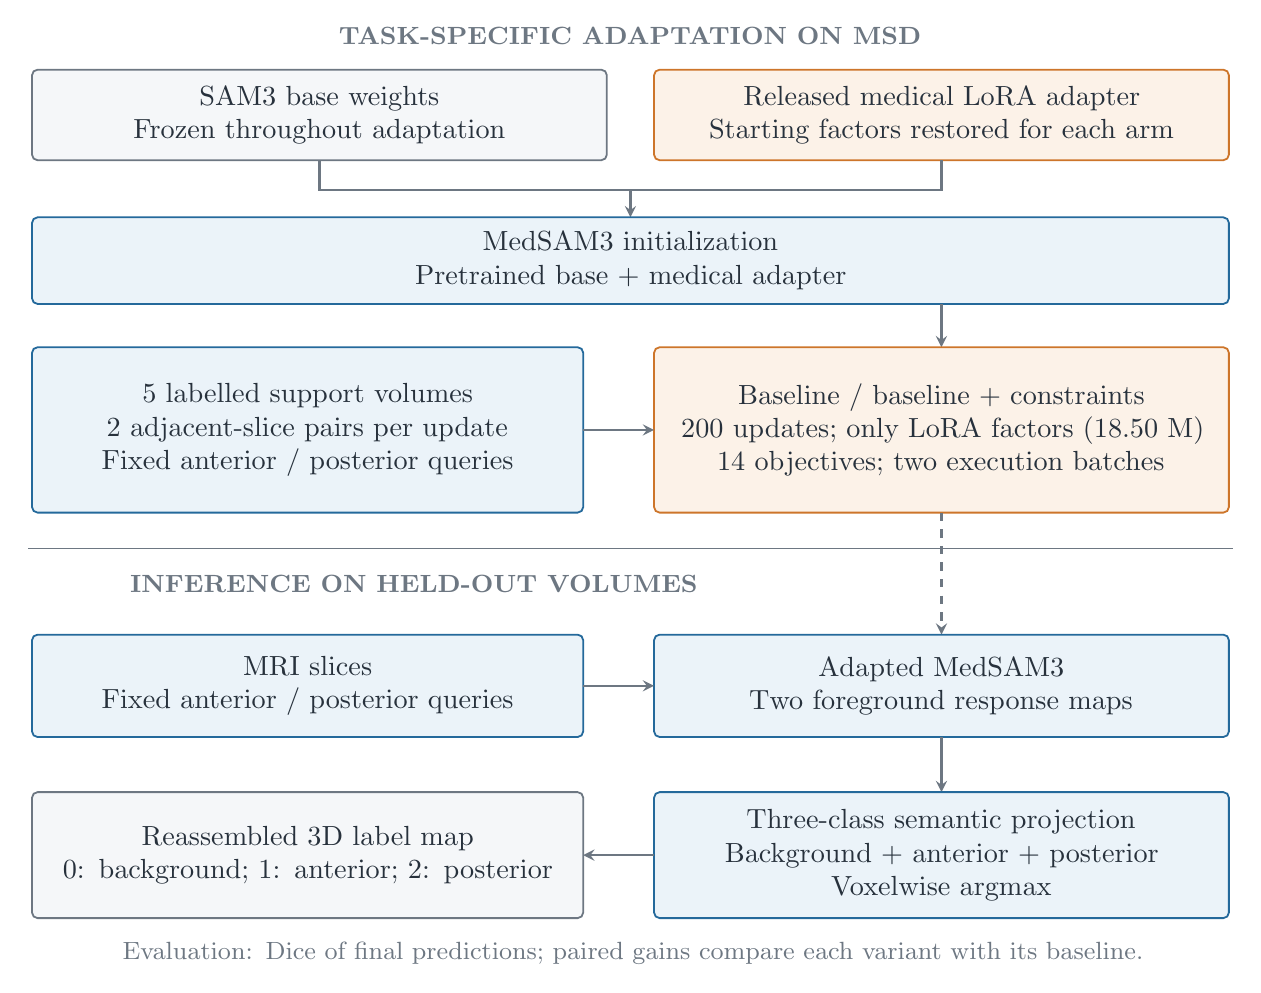
\begin{tikzpicture}[x=1cm,y=-1cm,font=\footnotesize,
  every node/.style={text=thesisInk},>=stealth]
\node[align=center,text width=15cm,inner sep=0pt,text=thesisGray,font=\fontsize{9}{11}\selectfont\bfseries] at (7.750,0.200) {TASK-SPECIFIC ADAPTATION ON MSD};
\draw[fill=thesisPaleGray,draw=thesisGray,line width=.65pt,rounded corners=2pt] (0.150,0.625) rectangle (7.450,1.775);
\node[align=center,text width=7.06cm,inner sep=0pt,text=thesisInk,font=\fontsize{10}{12}\selectfont] at (3.800,1.200) {SAM3 base weights\\Frozen throughout adaptation};
\draw[fill=thesisPaleOrange,draw=thesisOrange,line width=.65pt,rounded corners=2pt] (8.050,0.625) rectangle (15.350,1.775);
\node[align=center,text width=7.06cm,inner sep=0pt,text=thesisInk,font=\fontsize{10}{12}\selectfont] at (11.700,1.200) {Released medical LoRA adapter\\Starting factors restored for each arm};
\draw[draw=thesisGray,line width=0.8pt,->] (3.800,1.775) -- (3.800,2.150) -- (7.750,2.150) -- (7.750,2.500);
\draw[draw=thesisGray,line width=0.8pt] (11.700,1.775) -- (11.700,2.150) -- (7.750,2.150);
\draw[fill=thesisPaleBlue,draw=thesisBlue,line width=.65pt,rounded corners=2pt] (0.150,2.500) rectangle (15.350,3.600);
\node[align=center,text width=14.959999999999999cm,inner sep=0pt,text=thesisInk,font=\fontsize{10}{12}\selectfont] at (7.750,3.050) {MedSAM3 initialization\\Pretrained base + medical adapter};
\draw[draw=thesisGray,line width=0.8pt,->] (11.700,3.600) -- (11.700,4.150);
\draw[fill=thesisPaleBlue,draw=thesisBlue,line width=.65pt,rounded corners=2pt] (0.150,4.150) rectangle (7.150,6.250);
\node[align=center,text width=6.76cm,inner sep=0pt,text=thesisInk,font=\fontsize{10}{12}\selectfont] at (3.650,5.200) {5 labelled support volumes\\2 adjacent-slice pairs per update\\Fixed anterior / posterior queries};
\draw[fill=thesisPaleOrange,draw=thesisOrange,line width=.65pt,rounded corners=2pt] (8.050,4.150) rectangle (15.350,6.250);
\node[align=center,text width=7.06cm,inner sep=0pt,text=thesisInk,font=\fontsize{10}{12}\selectfont] at (11.700,5.200) {Baseline / baseline + constraints\\200 updates; only LoRA factors (18.50 M)\\14 objectives; two execution batches};
\draw[draw=thesisGray,line width=0.8pt,->] (7.150,5.200) -- (8.050,5.200);
\draw[draw=thesisGray,line width=0.3pt] (0.100,6.700) -- (15.400,6.700);
\node[align=center,text width=9.5cm,inner sep=0pt,text=thesisGray,font=\fontsize{9}{11}\selectfont\bfseries] at (5.000,7.150) {INFERENCE ON HELD-OUT VOLUMES};
\draw[draw=thesisGray,line width=0.8pt,->,dashed] (11.700,6.250) -- (11.700,7.800);
\draw[fill=thesisPaleBlue,draw=thesisBlue,line width=.65pt,rounded corners=2pt] (0.150,7.800) rectangle (7.150,9.100);
\node[align=center,text width=6.76cm,inner sep=0pt,text=thesisInk,font=\fontsize{10}{12}\selectfont] at (3.650,8.450) {MRI slices\\Fixed anterior / posterior queries};
\draw[fill=thesisPaleBlue,draw=thesisBlue,line width=.65pt,rounded corners=2pt] (8.050,7.800) rectangle (15.350,9.100);
\node[align=center,text width=7.06cm,inner sep=0pt,text=thesisInk,font=\fontsize{10}{12}\selectfont] at (11.700,8.450) {Adapted MedSAM3\\Two foreground response maps};
\draw[draw=thesisGray,line width=0.8pt,->] (7.150,8.450) -- (8.050,8.450);
\draw[draw=thesisGray,line width=0.8pt,->] (11.700,9.100) -- (11.700,9.800);
\draw[fill=thesisPaleBlue,draw=thesisBlue,line width=.65pt,rounded corners=2pt] (8.050,9.800) rectangle (15.350,11.400);
\node[align=center,text width=7.06cm,inner sep=0pt,text=thesisInk,font=\fontsize{10}{12}\selectfont] at (11.700,10.600) {Three-class semantic projection\\Background + anterior + posterior\\Voxelwise argmax};
\draw[fill=thesisPaleGray,draw=thesisGray,line width=.65pt,rounded corners=2pt] (0.150,9.800) rectangle (7.150,11.400);
\node[align=center,text width=6.76cm,inner sep=0pt,text=thesisInk,font=\fontsize{10}{12}\selectfont] at (3.650,10.600) {Reassembled 3D label map\\0: background; 1: anterior; 2: posterior};
\draw[draw=thesisGray,line width=0.8pt,->] (8.050,10.600) -- (7.150,10.600);
\node[align=center,text width=15.3cm,inner sep=0pt,text=thesisGray,font=\fontsize{9}{11}\selectfont] at (7.750,11.850) {Evaluation: Dice of final predictions; paired gains compare each variant with its baseline.};
\end{tikzpicture}
\caption{MedSAM3 adaptation and inference on MSD. Training changes only
the medical LoRA factors using five support crops per fold. The two
fixed queries produce foreground responses, which are combined with
background to obtain mutually exclusive labels. Held-out masks are used
for evaluation and supply no localization prompts.}
\label{fig:medsam3-workflow}
\end{figure}

\paragraph{MedSAM3 on ADNI.}\label{sec:medsam-adni-methods}
Each fold uses two labelled crops from two subjects and 54 held-out
crops from 27 other subjects. Folds 0 and 3 share their two support
crops; fold 1 shares one and changes the other. Only three distinct
support crops occur across the study. These folds vary the evaluation
partition, but do not provide three independent draws of a training set.

The medical initialization, 200-update schedule and intensity scaling
follow the MSD protocol. ADNI retains its stored array orientation and
uses the single query \emph{hippocampus}. The binary projection combines
the foreground response with its complement. Bands and edges supervise
the hippocampus mask, without a second background-mask average.
SDF uses unit array voxels, and depth uses source-axis geometry without
an inferred anatomical orientation.

These update budgets describe additional task adaptation and exclude
pretraining. They do not provide a FLOP match with the conventional
studies. Exact optimizer settings, calibration rules, fold and seed
identifiers, and execution environments are retained in
Appendix~\ref{sec:adaptation-implementation}. Runtime comparisons keep
their recorded scope; a training-loop timer is not an end-to-end
adaptation cost.

\subsection{Evaluation Measures}
\label{sec:evaluation-methods}

Dice serves two distinct roles. During training, a differentiable soft
Dice loss contributes to the architecture-specific optimization
objective. During evaluation, hard Dice measures overlap between the
final discrete predictions and reference labels. Every Dice score in
the results figures and tables uses this second definition, including scores on the
training support set. Validation Dice uses held-out examples;
training-set Dice uses examples supplied during fitting. Neither score
contains focal, cross-entropy, box, presence or spatial-constraint loss
terms, and neither is the value of the Dice loss used during training.

Voxelwise argmax defines the predicted label. For reference region
$Y_{i,c}$ and prediction $\widehat Y_{i,c}$, hard class Dice is
\begin{equation}
 D_{i,c}=\frac{2|Y_{i,c}\cap\widehat Y_{i,c}|}
 {|Y_{i,c}|+|\widehat Y_{i,c}|}.
\label{eq:reported-hard-dice}
\end{equation}
A present reference class with no predicted voxels scores zero.
The MSD volume score is the mean anterior/posterior Dice,
$D_i=(D_{i,A}+D_{i,P})/2$, and the ADNI volume score is hippocampus Dice. Geological evaluation
uses salt Dice.
Background is excluded from these primary metrics. Volumes receive
equal weight in a run mean. Section~\ref{sec:background-dice-results}
adds background and all-class Dice as complementary measures on
the same predictions, retaining this order of averaging.

Let $\overline D_{m,j,f,s}$ denote the mean volume Dice in a run with
model $m$, objective $j$, fold $f$ and seed $s$. Subscript
$\mathrm{base}$ identifies its matched baseline. Their paired change is
\begin{equation}
 \Delta_{m,j,f,s}=100\left(
 \overline D_{m,j,f,s}-\overline D_{m,\mathrm{base},f,s}\right).
\label{eq:paired-reported-gain}
\end{equation}
Dice is reported on a percentage scale and differences in percentage
points. Reported standard deviations are sample standard deviations across
the three seed-averaged fold means; paired-gain dispersions use the three
fold-mean differences. Positive-change counts use all nine matched
fold/seed cells. Each figure or table identifies its reduction explicitly.
These standard deviations are not confidence intervals over independent datasets: seeds share data,
training pools overlap and configuration selection is exploratory.
Dispersion across cases is identified separately from dispersion
across fold/seed cells.

A confusion matrix counts how often each reference class is assigned each
predicted class. The pretrained-model matrices use reference classes as rows
and predicted classes as columns. For MSD, four disjoint errors are counted:
background predicted as foreground, foreground predicted as background,
anterior predicted as posterior, and posterior predicted as anterior. Their
sum gives all incorrectly labelled voxels. Conventional-run error counts
pool the full validation grid before averaging runs. MedSAM3 tables average
errors per crop within each run and then weight folds equally. All counts
cover the complete prediction, including voxels outside the boundary bands.
SAM3 FN/FP are likewise averaged per held-out volume within a run, then over
seeds and folds; each run contains 96 validation volumes. Binary ADNI and
GeoFWI3D have no A/P swaps. The different error-count reductions are
labelled and are not compared as if they had the same denominator.

\clearpage

\section{Results and Analysis}
\label{sec:results}

Spatial supervision improves the best observed mean Dice in every model
and dataset studied, but its benefit depends on the objective and training
setting. This chapter presents those principal comparisons and examines
what the improvements mean. Complete aggregate results, including unsuccessful configurations,
and a compact fold summary are retained in Appendix~\ref{sec:extended-results};
the electronic supplement preserves every run and fold record.

The aggregate charts compare a baseline with the objective that has the highest
mean validation Dice in the same study. Selection uses these validation
results, so the comparisons are descriptive rather than independent tests
of an optimal method. Dice is reported in percent and gains in percentage
points (pp); all gains use the corresponding matched baseline.

\subsection{Spatial Supervision When Training from Scratch}
\label{sec:geo-results}\label{sec:main-msd-results}\label{sec:adni-results}

Figure~\ref{fig:scratch-key-results} brings the three datasets together.
The consistent pattern is an improvement over each model's own baseline.
The size of that improvement varies considerably, even among models
trained on the same data.

\begin{figure}[htbp]
\centering\setstretch{1.05}
% Cached vector figure; editable source: figures/source/scratch-key-results.tikz
\includegraphics{figures/compiled/scratch-key-results.pdf}
\caption{Training from scratch: baseline and the highest-mean tested
spatial objective for each model and dataset. Whiskers show the sample
standard deviation of three seed-averaged fold means; they are not
confidence intervals. Right-hand labels give paired gains from unrounded
scores. Foreground Dice averages anterior and posterior on MSD and measures
the single target class on the binary tasks. Panels share a score scale,
but their task and budget differences preclude a direct dataset ranking.
Complete objective scores and selected combinations are in
Appendix~\ref{sec:complete-result-tables}.}
\label{fig:scratch-key-results}
\label{fig:geo-key-results}\label{fig:msd-key-results}\label{fig:adni-key-results}
\end{figure}

The medical comparisons illustrate why absolute accuracy and improvement
must be distinguished. On MSD, SwinUNETR gains almost twelve points, yet
the compact U-Net reaches the highest Dice, 80.00\%. A large gain can
therefore reflect the correction of a weak short-budget baseline without
producing the most accurate model. On ADNI, nnU-Net starts from the
strongest baseline and retains the highest score, although its improvement
is only about one point.

The geological results extend the positive pattern beyond medical images.
The compact U-Net again reaches the highest score, while nnU-Net benefits
most from the added supervision. This is evidence that the approach can
help in both domains under the tested procedures. It does not establish
that one domain benefits more: the geological and medical comparisons
use different budgets and task definitions.

No single constraint combination explains all these gains. Boundary
membership alone improves every model mean across the three datasets,
but other additions can reduce accuracy. For example, signed-distance
supervision alone lowers the MSD nnU-Net mean by about two points.
The useful conclusion is therefore that annotation geometry can improve
learning when its contribution is tested within the chosen training
recipe. Adding more terms is not reliably better. The objective-level
comparisons, near ties and negative outcomes are documented in
Appendix~\ref{sec:secondary-objective-results}.

\FloatBarrier
\subsection{Spatial Supervision During Pretrained Adaptation}
\label{sec:sam3-results}\label{sec:medsam-results}\label{sec:medsam-adni-results}

The adaptation experiments ask whether the same idea remains useful when
the model already has a pretrained representation. Figure~\ref{fig:adaptation-key-results}
shows improvements in all three studies: SAM3 reaches 72.76\% Dice on
GeoFWI3D, while MedSAM3 reaches 81.73\% on MSD and 80.85\% on ADNI.
The largest improvement is on MSD, where the gain over the matched
adapted baseline exceeds five percentage points.

\begin{figure}[htbp]\centering
% Cached vector figure; editable source: figures/source/adaptation-key-results.tikz
\includegraphics{figures/compiled/adaptation-key-results.pdf}
\caption{Pretrained adaptation:
baseline and the highest-mean tested objective, with fold-level standard
deviations. The MSD baseline is matched to the execution batch of the
all-term variant. $B,E,S,D$ denote bands, edges, signed distance and depth
supervision. The studies use different support sizes and update budgets;
the figure compares each model with its own baseline. Full results are in
Appendix~\ref{sec:complete-result-tables}.}
\label{fig:adaptation-key-results}
\end{figure}

Spatial supervision consequently remains useful beyond learning from
scratch. The improvement is present in every fold mean for each selected
configuration, although the SAM3 gain varies more across support
partitions. The medical gains are positive in every matched run; SAM3
has one negative pair. These patterns support a benefit under the
evaluated adaptation conditions, without implying that every new support
set would produce the same change.

The preferred objective again depends on the task. SAM3 benefits most
from bands, edges and depth supervision; including signed distance lowers
its mean. MedSAM3 on MSD reaches its highest mean with all four terms,
whereas ADNI has closely ranked alternatives. The studies also differ in
initialization, support size and update budget, so their scores cannot
isolate the effect of medical pretraining or establish a model ranking at
equal resources. For MSD, comparisons retain the control from each
variant's execution batch; the complete matched results are in
Table~\ref{tab:medsam-msd-noaug}.

\FloatBarrier
\subsection{What the Overlap Improvements Mean}
\label{sec:error-analysis}\label{sec:capped-errors-resources}
\label{sec:background-dice-results}

Higher Dice does not mean that every kind of error becomes less frequent.
Across the adaptation studies, the selected constraints recover more of
the target structure but also label more surrounding voxels as foreground.
On MSD, fewer anterior/posterior exchanges accompany this tradeoff.
The models trained from scratch show a less uniform pattern: some mainly
reduce missed foreground, others mainly reduce unwanted extension. These
differences matter when deciding which errors an application can tolerate;
error changes are summarized in Appendix~\ref{sec:complete-error-tables};
complete counts for every objective are in the electronic supplement.

Including background in the Dice average provides a complementary check on
the overlap gains. All-class Dice gives equal weight to each class:
background, anterior and posterior on MSD, or background and the single
foreground class on the binary tasks.
Figure~\ref{fig:metric-sensitivity-key-results} shows that the selected
adaptation objectives improve both foreground and background Dice. The same
holds for the selected conventional models. Background scores already lie
close to their ceiling, so their changes are much smaller. Giving background
equal class weight raises the absolute average while reducing the size of
the improvement.

\begin{figure}[htbp]\centering\setstretch{1.05}
% Cached vector figure; editable source: figures/source/metric-sensitivity-key-results.tikz
\includegraphics{figures/compiled/metric-sensitivity-key-results.pdf}
\caption{The same adaptation
predictions assessed in three ways. Bars show mean gains for the objectives
in Figure~\ref{fig:adaptation-key-results}, calculated from the unrounded
archive aggregates. Including the already high-scoring background reduces
the gain in the class average, while preserving its positive direction.
These are complementary measurements of the same runs. The exact
aggregation, absolute scores and checks across all recoverable objectives
are in Appendix~\ref{sec:metric-sensitivity-details}.}
\label{fig:metric-sensitivity-key-results}
\end{figure}

The main conclusion survives this change of measure: across all recoverable
comparisons, the sign of the mean effect and the highest-mean objective
in each study are unchanged. A few small individual effects and secondary
rankings differ. Appendix~\ref{sec:metric-sensitivity-details} gives the
full checks and archive coverage. The earlier MSD MedSAM3 bands and
bands-plus-edges comparisons retain complete foreground results, but lack
recoverable background scores.

Figure~\ref{fig:qualitative-typical} makes these differences visible through
matched image, reference and prediction panels. The examples come from
six short, matched reproductions of SAM3 on GeoFWI3D and MedSAM3 on MSD
and ADNI, performed because the original trained adapters and predictions
were no longer available. They illustrate the segmentation behaviour;
the original three-fold, three-seed studies remain the basis of the
aggregate results above. Appendix~\ref{sec:qualitative-predictions}
documents the case selection and differences from the original run scores.

\begin{figure}[p]
\centering
\includegraphics[width=\linewidth]{figures/qualitative/typical-predictions.png}
\caption{Typical held-out examples from the qualitative reproductions:
SAM3 on GeoFWI3D and MedSAM3 on MSD and ADNI. Each case is the middle entry after sorting by paired Dice change,
using the higher of the two central entries for an even-sized validation set. Columns use the
same image and slice, selected by maximum reference foreground area along
the third stored array axis. Blue denotes salt, anterior hippocampus or
whole hippocampus, respectively; orange denotes posterior hippocampus on
MSD. Scores describe the whole volume, with anterior/posterior Dice
averaged on MSD, rather than the displayed slice. The constrained
objectives are $B+E+D$, $B+E+S+D$ and $E+S+D$, respectively.
Adverse cases are shown in Appendix~\ref{sec:qualitative-predictions};
largest-gain cases are retained in the electronic supplement.}
\label{fig:qualitative-typical}
\end{figure}

The examples show local changes rather than a wholesale change in the
predicted object. In the MSD view, the constrained prediction recovers
more of the posterior region; in the ADNI view it extends towards parts
of the reference missed by the baseline. Contour disagreements remain in
both. Across the full volumes of these three typical cases, missed
foreground decreases while extra foreground increases. The adverse
examples in the appendix show that this tradeoff can instead lower Dice.
A single slice cannot explain every change in a volume score, and neither
these images nor overlap measurements establish downstream usefulness.
Surface-distance evaluation and expert assessment remain necessary to
address that question.

\FloatBarrier
\subsection{Limits of the Findings}
\label{sec:limitations}\label{sec:experimental-limitations}

The results concern limited training budgets, prepared hippocampus crops
and synthetic geological volumes. They establish benefits within those
settings; persistence after substantially longer training and transfer
to uncropped medical images or measured seismic data remain open.
Small support sets and overlap between some support partitions also
limit conclusions about sensitivity to the annotated examples available.

The comparisons evaluate complete calibrated objectives. In particular,
depth supervision adds a class loss as well as spatial weighting, so
a matched unweighted control is needed to distinguish those contributions.
Closely ranked combinations should likewise be treated as alternatives
within the observed variation rather than evidence of a unique optimum.

The MSD annotation audit gives a related caution about the knowledge encoded
in a constraint. Neither a single coronal separating plane nor a rule based
on separate foreground regions appearing in a slice reproduces every
annotated anterior/posterior transition. The thesis therefore supervises the
stored class boundary rather than imposing either proxy universally. The
detailed checks and their relation to the original annotation protocols are
in Appendix~\ref{sec:annotation-results}; they do not establish that the
original anatomical tracing was incorrect.

\clearpage

\section{Conclusions}\label{sec:conclusions}

This thesis examined whether segmentation models can make better use of
limited annotations by explicitly supervising their spatial information.
The LTN/logLTN formulation connects four properties of the label maps to
trainable losses: membership near boundaries, agreement between
neighbouring labels, classwise distance and supervision across depth
layers. These terms require no additional manual labels and leave the
model's inference inputs unchanged.

The experiments support this approach under the evaluated data and
training budgets. Benefits occur in both geological and medical tasks,
and in models trained from scratch as well as adapted pretrained models.
Their size and the preferred objective depend on the learning setting.
The contribution is therefore a set of explicitly defined spatial
objectives and evidence of where they help, rather than a universally
preferred combination. The full comparisons, error tradeoffs and limits
of this evidence are discussed in Chapter~\ref{sec:results}.

\subsection{Future Research Directions}\label{sec:future-work}
\label{sec:pending-results}

The first priority is an independent evaluation with model,
objective and data-selection choices fixed in advance. New participants
and imaging collections would test whether the gains extend beyond the
datasets used to develop these recipes. Varying annotation and compute
budgets, including longer training and matched data exposure, would
show when constraints accelerate learning and when they improve the
accuracy ultimately reached. An unweighted classification control is
also needed to separate depth weighting from the benefit of additional
class supervision.

Surface-distance evaluation would complement Dice by measuring how far
predicted boundaries lie from the reference contours. Expert assessment
could examine whether the remaining contour and internal class-assignment
errors matter for the intended application. Together, these evaluations
would extend the analysis beyond overlap scores and visual comparisons.

Hippocampal subfield datasets offer a further test of spatial knowledge.
The Montreal Neurological Institute hippocampal subfield dataset
(MNI-HISUB25) and the atlas of Winterburn \emph{et al.}\ contain finer
anatomical subdivisions
\cite{kulaga2015subfields,winterburn2013atlas}; the dataset of
Jafari \emph{et al.}\ adds a different clinical population
\cite{jafari2011dataset}. None is evaluated here. Their annotation
protocols could support statements about shared interfaces, relative
position and continuity of thin structures. Such relations would
require expert validation and tolerances for anatomical variation.

For the MSD anterior/posterior division, expert landmark annotations
and multiplanar images could support an uncertain transition region
around the uncal apex. This would allow a comparison between
landmark-guided supervision and the existing classwise terms without
assuming that one fixed cut describes every mask.

Pretrained adaptation could be extended by varying the support-set
composition, adapter capacity and amount of neighbouring-slice context.
Accuracy and additional computation should be reported together.
Adaptive constraint weights are another possibility, but their value
would need controlled comparisons with the fixed calibration used here.
These studies would identify which changes add useful supervision and
which mainly add training cost.

\clearpage

% Embedded bibliography for the self-contained thesis document.
% The Overleaf template can instead use ref.bib with its existing
% \addbibresource{ref.bib} and \printbibliography commands.
\renewcommand{\refname}{Bibliography}
\phantomsection
\addcontentsline{toc}{section}{Bibliography}
\begin{thebibliography}{99}
\bibitem{wang2021annotation}
S.~Wang et al., ``Annotation-efficient deep learning for automatic medical
image segmentation,'' \emph{Nature Communications}, vol.~12, article~5915,
2021. \url{https://doi.org/10.1038/s41467-021-26216-9}.

\bibitem{swaminadhan2026geofwi3d}
S.~Swaminadhan et al., ``GeoFWI3D: Large-scale 3D Velocity Model Dataset for
Deep Learning-assisted Seismic Imaging,'' arXiv:2610.01033, 2026.
\url{https://arxiv.org/abs/2610.01033}.

\bibitem{niaAlzheimerBrain}
National Institute on Aging, ``What Happens to the Brain in Alzheimer's
Disease?'' Accessed 9 October 2026.
\url{https://www.nia.nih.gov/health/alzheimers-causes-and-risk-factors/what-happens-brain-alzheimers-disease}.

\bibitem{simpson2019dataset}
A.~L. Simpson et al., ``A large annotated medical image dataset for the
development and evaluation of segmentation algorithms,'' arXiv:1902.09063,
2019. \url{https://arxiv.org/abs/1902.09063}.

\bibitem{pruessner2000volumetry}
J.~C. Pruessner et al., ``Volumetry of hippocampus and amygdala with
high-resolution MRI and three-dimensional analysis software: minimizing
the discrepancies between laboratories,'' \emph{Cerebral Cortex},
vol.~10, no.~4, pp.~433--442, 2000.
\url{https://doi.org/10.1093/cercor/10.4.433}.

\bibitem{woolard2012asymmetry}
A.~A. Woolard and S.~Heckers, ``Anatomical and functional correlates of
human hippocampal volume asymmetry,'' \emph{Psychiatry Research:
Neuroimaging}, vol.~201, no.~1, pp.~48--53, 2012.
\url{https://doi.org/10.1016/j.pscychresns.2011.07.016}.

\bibitem{adniStudy}
Alzheimer's Disease Neuroimaging Initiative, ``ADNI: Alzheimer's Disease
Neuroimaging Initiative.'' Accessed 9 October 2026.
\url{https://adni.loni.usc.edu/}.

\bibitem{badreddine2022logic}
S.~Badreddine, A.~d'Avila Garcez, L.~Serafini and M.~Spranger,
``Logic Tensor Networks,'' \emph{Artificial Intelligence}, vol.~303,
article~103649, 2022.
\url{https://doi.org/10.1016/j.artint.2021.103649}.

\bibitem{badreddine2023logltn}
S.~Badreddine, L.~Serafini and M.~Spranger,
``logLTN: Differentiable Fuzzy Logic in the Logarithm Space,''
arXiv:2306.14546, 2023. \url{https://arxiv.org/abs/2306.14546}.

\bibitem{liu2025medsam3}
A.~Liu et al., ``MedSAM3: Delving into Segment Anything with Medical
Concepts,'' arXiv:2511.19046v1, 2025.
\url{https://arxiv.org/abs/2511.19046v1}.

\bibitem{nifti1fields}
Neuroimaging Informatics Technology Initiative, ``NIfTI-1 Fields.''
Accessed 9 October 2026.
\url{https://nifti.nimh.nih.gov/nifti-1/documentation/nifti1fields.html}.

\bibitem{cicek2016unet}
\"O.~\c{C}i\c{c}ek, A.~Abdulkadir, S.~S. Lienkamp, T.~Brox and
O.~Ronneberger, ``3D U-Net: Learning Dense Volumetric Segmentation from
Sparse Annotation,'' arXiv:1606.06650, 2016.
\url{https://arxiv.org/abs/1606.06650}.

\bibitem{ronneberger2015unet}
O.~Ronneberger, P.~Fischer and T.~Brox, ``U-Net: Convolutional Networks
for Biomedical Image Segmentation,'' arXiv:1505.04597, 2015.
\url{https://arxiv.org/abs/1505.04597}.

\bibitem{milletari2016vnet}
F.~Milletari, N.~Navab and S.-A.~Ahmadi, ``V-Net: Fully Convolutional
Neural Networks for Volumetric Medical Image Segmentation,''
arXiv:1606.04797, 2016. \url{https://arxiv.org/abs/1606.04797}.

\bibitem{isensee2021nnunet}
F.~Isensee, P.~F. Jaeger, S.~A.~A. Kohl, J.~Petersen and K.~H. Maier-Hein,
``nnU-Net: a self-configuring method for deep learning-based biomedical
image segmentation,'' \emph{Nature Methods}, vol.~18, pp.~203--211, 2021.
\url{https://doi.org/10.1038/s41592-020-01008-z}.

\bibitem{vaswani2017attention}
A.~Vaswani et al., ``Attention Is All You Need,'' arXiv:1706.03762,
2017. \url{https://arxiv.org/abs/1706.03762}.

\bibitem{hatamizadeh2021unetr}
A.~Hatamizadeh et al., ``UNETR: Transformers for 3D Medical Image
Segmentation,'' arXiv:2103.10504, 2021.
\url{https://arxiv.org/abs/2103.10504}.

\bibitem{liu2021swin}
Z.~Liu et al., ``Swin Transformer: Hierarchical Vision Transformer using
Shifted Windows,'' arXiv:2103.14030, 2021.
\url{https://arxiv.org/abs/2103.14030}.

\bibitem{hatamizadeh2022swin}
A.~Hatamizadeh, V.~Nath, Y.~Tang, D.~Yang, H.~Roth and D.~Xu,
``Swin UNETR: Swin Transformers for Semantic Segmentation of Brain Tumors
in MRI Images,'' arXiv:2201.01266, 2022.
\url{https://arxiv.org/abs/2201.01266}.

\bibitem{kervadec2019boundary}
H.~Kervadec, J.~Bouchtiba, C.~Desrosiers, E.~Granger, J.~Dolz and
I.~Ben Ayed, ``Boundary loss for highly unbalanced segmentation,''
in \emph{Proceedings of The 2nd International Conference on Medical
Imaging with Deep Learning}, Proceedings of Machine Learning Research,
vol.~102, pp.~285--296, 2019.
\url{https://proceedings.mlr.press/v102/kervadec19a.html}.

\bibitem{oktay2017anatomically}
O.~Oktay et al., ``Anatomically Constrained Neural Networks (ACNN):
Application to Cardiac Image Enhancement and Segmentation,''
arXiv:1705.08302, 2017. \url{https://arxiv.org/abs/1705.08302}.

\bibitem{shit2021cldice}
S.~Shit et al., ``clDice---A Novel Topology-Preserving Loss Function
for Tubular Structure Segmentation,'' in \emph{Proceedings of the
IEEE/CVF Conference on Computer Vision and Pattern Recognition}, 2021.
\url{https://doi.org/10.1109/CVPR46437.2021.01629}.

\bibitem{bergamin2025integrating}
L.~Bergamin, G.~M. Dimitri and F.~Aiolli, ``Integrating Background
Knowledge in Medical Semantic Segmentation with Logic Tensor Networks,''
arXiv:2509.22399, 2025. \url{https://arxiv.org/abs/2509.22399}.

\bibitem{kirillov2023segment}
A.~Kirillov et al., ``Segment Anything,'' arXiv:2304.02643, 2023.
\url{https://arxiv.org/abs/2304.02643}.

\bibitem{ma2024medsam}
J.~Ma, Y.~He, F.~Li, L.~Han, C.~You and B.~Wang,
``Segment anything in medical images,'' \emph{Nature Communications},
vol.~15, article~654, 2024.
\url{https://doi.org/10.1038/s41467-024-44824-z}.

\bibitem{carion2025sam3}
N.~Carion et al., ``SAM 3: Segment Anything with Concepts,''
arXiv:2511.16719v1, 2025. \url{https://arxiv.org/abs/2511.16719v1}.

\bibitem{hu2021lora}
E.~J. Hu et al., ``LoRA: Low-Rank Adaptation of Large Language Models,''
arXiv:2106.09685, 2021. \url{https://arxiv.org/abs/2106.09685}.
\bibitem{harpReleasedLabels}
EADC--ADNI Harmonized Protocol, ``Released Images: Final Release.''
Accessed 11 October 2026.
\url{https://www.hippocampal-protocol.net/SOPs/labels.php}.

\bibitem{kulaga2015subfields}
J.~Kulaga-Yoskovitz et al., ``Multi-contrast submillimetric 3 Tesla
hippocampal subfield segmentation protocol and dataset,''
\emph{Scientific Data}, vol.~2, article~150059, 2015.
\url{https://doi.org/10.1038/sdata.2015.59}.

\bibitem{winterburn2013atlas}
J.~L. Winterburn et al., ``A novel in vivo atlas of human hippocampal
subfields using high-resolution 3 T magnetic resonance imaging,''
\emph{NeuroImage}, vol.~74, pp.~254--265, 2013.
\url{https://doi.org/10.1016/j.neuroimage.2013.02.003}.

\bibitem{jafari2011dataset}
K.~Jafari-Khouzani, K.~V. Elisevich, S.~Patel and H.~Soltanian-Zadeh,
``Dataset of magnetic resonance images of nonepileptic subjects and
temporal lobe epilepsy patients for validation of hippocampal
segmentation techniques,'' \emph{Neuroinformatics}, vol.~9, no.~4,
pp.~335--346, 2011. \url{https://doi.org/10.1007/s12021-010-9096-4}.

\end{thebibliography}

\clearpage
\appendix

\section{Numerical and Implementation Details}
\label{sec:technical-details}

This appendix records the numerical conventions and training settings
needed to reproduce the methods. Extended derivations and execution
records are supplied in the electronic supplement described in
Appendix~\ref{sec:evidence-register}.

\subsection{Stable Loss Evaluation and Derivatives}
\label{sec:band-implementation-details}

For a class group $F$ and its complement $\overline F$, let $z_U$
collect the logits for classes in a set $U$. Define
$\operatorname{LSE}(z_U)=\log\sum_{c\in U}\exp z_c$,
$\sigma(s)=1/(1+\exp(-s))$ and
$\operatorname{softplus}(s)=\log(1+\exp s)$. The grouped logit and
stable binary cross-entropy are
\begin{align}
s_F&=\operatorname{LSE}(z_F)-\operatorname{LSE}(z_{\overline F}),
 &\sigma(s_F)&=\sum_{c\in F}p_c,\label{eq:grouped-predicate-logit}\\
e_i(v)&=h_i(v)\operatorname{softplus}(-s_i(v))
 +(1-h_i(v))\operatorname{softplus}(s_i(v)).&&\label{eq:band-stable-bce}
\end{align}
Grouped logits and losses use float32; classwise log-probabilities use
log-softmax. Optional focal factors and neighbour-count weights are
disabled. The band count constant is $\varepsilon=10^{-6}$. Adding it
to a nonempty count multiplies the exact side mean by
$\rho_i^s=n_i^s/(n_i^s+\varepsilon)$; the implemented case loss is
$\tfrac12\sum_s\rho_i^s b_i^s$, where $b_i^s$ is that side's mean
negative log-truth. Both bands must be nonempty for a case to enter the
mean. If none is valid, a zero connected to the logits gives zero
gradient. These conventions retain the implemented value rather than
silently replacing stabilized sums by exact means.
In terms of the inner and outer statement satisfactions, the exact
identity is
\begin{equation}
\exp(-\mathcal L_{B,i})=
\mathcal G_\theta(\Phi_i^{\rm in})^{\rho_i^{\rm in}/2}
\mathcal G_\theta(\Phi_i^{\rm out})^{\rho_i^{\rm out}/2}.
\label{eq:balanced-band-satisfaction}
\end{equation}

For edges, $\mathcal N_i^B(u)$ contains the neighbours of $u$ in the
selected pair set, $n_i^E$ is the number of selected pairs and
$\delta_i=q_i-h_i$. Differentiation gives
\begin{equation}
\begin{aligned}
\frac{\partial\mathcal L_{E,i}}{\partial q_i(u)}
 &=\frac{2}{n_i^E}\sum_{v\in\mathcal N_i^B(u)}
     (\delta_i(u)-\delta_i(v)),\\
\frac{\partial\mathcal L_{E,i}}{\partial s_i(u)}
 &=q_i(u)(1-q_i(u))\frac{\partial\mathcal L_{E,i}}{\partial q_i(u)}.
\end{aligned}\label{eq:edge-logit-gradient}
\end{equation}
The first line is a graph Laplacian: it sums residual differences with
neighbours. The sigmoid factor reduces the logit gradient near zero or
one. For the MSD signed-distance term, set $\bar\varphi_{i,0}=0$ and
$\bar\varphi_{i,c}=\varphi_{i,c}$ for $c\in\{A,P\}$. Then
\begin{equation}
\frac{\partial\mathcal L_{\mathrm{SDF},i}}{\partial z_{i,k}(v)}
=\frac{p_{i,k}(v)}{2|\Omega_i|}
 \left[\bar\varphi_{i,k}(v)-\sum_{c\in\mathcal C}
 p_{i,c}(v)\bar\varphi_{i,c}(v)\right].
\label{eq:sdf-logit-gradient}
\end{equation}
The fixed annotation offset does not change this derivative. Case
averaging, calibrated coefficients and schedules then apply as in the
main objective.

\subsection{Distance Fields and Observation Geometry}
\label{sec:sdf-construction-details}

For a nonempty, non-full class mask $M$, let $d(v,U)$ be the Euclidean
distance from voxel centre $v$ to the nearest centre in $U$. The field
used in the implementation is
\begin{equation}
\varphi^{\rm raw}(v)=
\begin{cases}
-(d(v,\Omega\setminus M)-\tfrac12), & v\in M,\\
d(v,M)-\tfrac12, & v\notin M,
\end{cases}
\qquad
\varphi(v)=\frac{\operatorname{clip}(\varphi^{\rm raw}(v),-8,8)}{8}.
\label{eq:sdf-half-voxel-field}
\end{equation}
The half-voxel shift places the interface between opposite-class
centres; it does not give an exact continuous-surface distance for every
boundary orientation. A missing class receives the constant field $+1$;
a full-grid class receives $-1$; both remain in the class reduction.
No exterior background frame is added. The conventional construction uses unit grid
spacing. Pretrained MSD uses its verified 1 mm spacing; ADNI and
GeoFWI3D use unit source-array coordinates. Clipping and normalization
retain these stated units.

For the MSD depth construction, $r_i(v)$ maps a voxel index to its
physical position. The foreground centroid and covariance are
\begin{equation}
\mu_i=\frac{1}{|M_i|}\sum_{v\in M_i}r_i(v),\qquad
\Sigma_i=\frac{1}{|M_i|}\sum_{v\in M_i}
(r_i(v)-\mu_i)(r_i(v)-\mu_i)^{\mathsf T}.
\label{eq:depth-centroid-covariance}
\end{equation}
The largest-eigenvalue eigenvector supplies the principal axis. Its
sign is oriented anteriorly, although reversing it leaves the projected
rightward normal unchanged. The eigenvalue gap is recorded as a
diagnostic. The surrounding region contains voxel centres within
8 mm of the foreground. Axis spacings are column norms of the affine
matrix $Q_i$; this distance calculation requires orthogonal axes.
Sheared affines, fewer than four foreground points, or a projected
normal of norm below 0.1 are rejected. ADNI's placeholder identity
affines establish neither anatomical orientation nor physical spacing;
its construction uses source-array coordinates in voxel units.

\paragraph{Geological crop faces.}\label{sec:geo-boundaries}
For axis lengths $N_{i,k}$, define
\begin{equation}
R_i^{(r)}=\{v\in\Omega_i:r\leq v_k\leq N_{i,k}-1-r, k=1,2,3\}.
\label{eq:geological-band-frame}
\end{equation}
The final UNETR recipe intersects both bands with $R_i^{(2)}$;
nnU-Net, SwinUNETR and the compact U-Net retain the zero-padded bands.
Band losses average the two stabilized side means and require both
sides to be nonempty. Edge pairs require both endpoints in the retained
band support; an exact pair mean is followed by a valid-case mean.
An empty valid-case set gives a differentiable zero. Signed distance
covers the full grid, including crop faces, with loss
$|\Omega_i|^{-1}\sum_v(p_{i,S}(v)-y_{i,S}(v))\varphi_{i,S}(v)$.

\paragraph{Earlier geological development check.}\label{sec:geo-development}
A separate UNETR check jointly changed frame exclusion and calibration,
obtaining 50.61\% versus 52.03\% Dice after 407
updates. It used one fold/seed pair and learning rate $5\times10^{-4}$;
the final recipe uses $6\times10^{-4}$. Its 1.42-point difference
cannot isolate the effect of frame exclusion and is excluded from the
final three-fold results.

\subsection{Sampled Volumetric Supervision}
\label{sec:sampled-pretrained-supervision}

Native three-dimensional masks define the supports before planes are
sampled. Let $Z_i$ be the number of planes, $k$ a uniformly sampled
anchor, and $\Omega_i^{(k)}$ its $N_i$ voxels. Band counts $n_{i,c}^s$
and edge counts $n_{i,c}^E$ refer to the full volume. For nonempty
supports, the anchor estimators are
\begin{align}
\widehat{\mathcal L}_{B,i,c}^{(k)}
 &=-\frac{Z_i}{2}\left[
 \frac{\sum_{v\in B_{i,c}^{\rm in}\cap\Omega_i^{(k)}}\log p_{i,c}(v)}{n_{i,c}^{\rm in}+\varepsilon}
 +\frac{\sum_{v\in B_{i,c}^{\rm out}\cap\Omega_i^{(k)}}\log(1-p_{i,c}(v))}{n_{i,c}^{\rm out}+\varepsilon}
 \right],\label{eq:medsam-sampled-band-loss}\\
\widehat{\mathcal L}_{E,i,c}^{(k)}
 &=\frac{Z_i}{n_{i,c}^E}\sum_{\{u,v\}\in\mathcal E_{i,c}^B(k)}
 (\delta_{i,c}(u)-\delta_{i,c}(v))^2,\label{eq:medsam-sampled-edge-loss}\\
\widehat{\mathcal L}_{S,i}^{(k)}
 &=\frac{1}{|C_+|N_i}\sum_{c\in C_+}\sum_{v\in\Omega_i^{(k)}}
 (p_{i,c}(v)-y_{i,c}(v))\varphi_{i,c}(v),\label{eq:medsam-sampled-sdf}\\
\widehat{\mathcal L}_{D,i}^{(k)}
 &=-Z_i\sum_{v\in\Omega_i^{(k)}}w_i(v)\log p_{i,y_i(v)}(v).
 \label{eq:medsam-sampled-depth}
\end{align}
Here $C_+$ is the foreground class set, $w_i$ sums to one over the
volume, and $\delta_{i,c}=p_{i,c}-y_{i,c}$. The edge set for anchor $k$
contains its in-plane pairs and the pairs to $k+1$, when that plane
exists. Every full-volume edge is assigned once. The baseline's
companion plane wraps from the last index to zero, but no edge joins
those two planes. For fixed predictions, averaging each estimator over
all $Z_i$ anchors recovers its full-volume loss and gradient.

MSD averages band and edge contributions over all three classes,
including background; ADNI and GeoFWI3D use the single foreground
mask. A class with an empty full-volume band side or edge set contributes
zero and retains its place in the class mean. An empty sampled support
does not change the full-volume denominator. Morphology uses zero
padding, so MSD background bands can reach crop faces. Volumes and
anchors are sampled uniformly; two adjacent-plane pairs are averaged
per optimizer update.

\subsection{Calibration and Activation Schedules}
\label{sec:detailed-calibration}

Conventional models calibrate gradients with respect to detached
float32 primary logits $z_i$, with $m_i$ entries. For case $i$, define
\begin{equation}
g_{i,0}=\nabla_{z_i}\mathcal L_{{\rm seg},i},\quad
g_{i,j}=\nabla_{z_i}\mathcal L_{j,i},\quad
\operatorname{RMS}(g)=\sqrt{m_i^{-1}\sum_{k=1}^{m_i}g_k^2}.
\label{eq:calibration-logit-gradients}
\end{equation}
The order is $B\to E\to S\to D$, omitting absent terms. If $K_j$
contains preceding terms, calibration uses
\begin{equation}
g_{i,<j}=g_{i,0}+\sum_{k\in K_j}\lambda_k g_{i,k},\quad
r_{i,j}=\frac{\operatorname{RMS}(g_{i,j})}{\operatorname{RMS}(g_{i,<j})},\quad
\lambda_j=\min\left\{\frac{\eta_a}{\operatorname{median}_i r_{i,j}},
\frac{\kappa_a}{Q_{0.95}(\{r_{i,j}\}_i)}\right\}.
\label{eq:constraint-calibrated-coefficient}
\end{equation}
The median target $\eta_a$ and percentile cap $\kappa_a$ control relative
gradient scale. Quantiles use linear interpolation and require finite
positive ratios. Adding vectors before measuring RMS retains their
directional interactions; adding norms would change the calibration.
Depth is calibrated against preceding terms at full strength even when
SDF activates later.

MSD and ADNI use all ten support cases after a baseline prefix of nine
updates for nnU-Net or 50 for the other models. Parameters, stored
network values and random-generator states remain unchanged during
the measurement. nnU-Net includes its primary deep-supervision weight;
coarser detached outputs contribute no logit derivative. The medical
settings are $(\eta_a,\kappa_a)=(0.6,0.75)$ for nnU-Net and
$(0.1,0.5)$ otherwise. GeoFWI3D uses all 19 training scenes, with
$(3.6,4.5)$ for nnU-Net, $(0.4,2.0)$ for UNETR and $(0.1,0.5)$
otherwise. These model-specific strengths followed exploratory comparisons.

For prefix $d_a$ and ramp length $w_a$, early terms use
$s_a(t)=\min\{1,\max\{0,(t-d_a)/w_a\}\}$, with $d_a=w_a=9$
for nnU-Net and 50 otherwise. SDF shares this ramp or starts near
five ninths of the nominal FLOP allowance, with a separate ramp of
the same length (Table~\ref{tab:sdf-activation-policies}). This policy
was developed using earlier MSD validation experiments and retained
for the campaigns; coefficient calibration itself uses support data
only. Learning-rate horizons remain fixed when costs change the number
of affordable updates.

\subsection{Compute Accounting and Model Settings}
\label{sec:detailed-resource-accounting}\label{sec:geological-budget-details}
\label{sec:implementation-tables}\label{sec:conventional-implementation}

The medical ceiling is 90 times the measured nnU-Net baseline update
cost of $355{,}293{,}896{,}301$ FLOPs:
\begin{equation}
C_{\max}=31{,}976.45066709\;\mathrm{GFLOPs}.
\label{eq:main-numerical-cap}
\end{equation}
Exploratory learning curves informed this short reference allowance.
The ledger charges forward computation, active losses, backward
computation and the optimizer, counting two FLOPs per
multiply--accumulate. Fixed-target construction, validation, loading
and storage are excluded; medical calibration is reported separately.
For GeoFWI3D, the retained cap is
\begin{equation}
C_{\rm train}+C_{\rm cal}\leq182{,}178.12654316\;\mathrm{GFLOPs}.
\label{eq:geological-compute-cap}
\end{equation}
It was defined as 152 times the original Dice-only nnU-Net update
profile of $1{,}198.540306205$ GFLOPs. The final Dice-plus-cross-entropy
baseline fits 151 updates. Geological evaluation, preflight diagnostics
and recipe development are excluded. Thus the two datasets' allowances
differ in both magnitude and treatment of calibration.

Let $d_a,d_a^S$ mark early and delayed activation, and let
$f_{a,0},f_{a,1},f_{a,2}$ be the measured update costs in the three
successive phases. With $[x]_+=\max(x,0)$, the training charge is
\begin{equation}
C_a(n)=f_{a,0}\min(n,d_a)
+f_{a,1}[\min(n,d_a^S)-d_a]_+
+f_{a,2}[n-d_a^S]_+.
\label{eq:piecewise-optimization-cost}
\end{equation}
The last integer update fitting the applicable ledger is admitted.
Delayed activation uses the boundary nearest five ninths of the
nominal cap after the early ramp, breaking ties toward the earlier
boundary. Attempted updates are charged even if a numerical failure
prevents a parameter change. Final states supply the reported scores;
there is no early stopping or validation-best checkpoint substitution.
With batch size one, completed epochs equal $\lfloor U/N\rfloor$
for $U$ updates and $N$ training cases; calibration does not add epochs.

The compact MONAI BasicUNet uses encoder widths $16,16,32,64,128$
and final decoder width 16, with pooling, transposed convolutions and
concatenated skips, without residual blocks or deep supervision.
The fixed nnU-Net has five stages of widths $32,64,128,256,320$,
three-dimensional kernels, instance normalization and leaky rectified
linear activations. UNETR has 12 blocks, embedding width 768, 12
attention heads and $16^3$ patches (64 tokens per $64^3$ medical crop),
with a residual convolutional decoder of base width 16. SwinUNETR
uses a hierarchical shifted-window encoder and convolutional decoder.
Constraints apply only to the primary output; nnU-Net's other supervised
resolutions keep their baseline losses.

nnU-Net uses polynomial learning-rate decay with exponent 0.9 and no
warmup. AdamW models warm up over 5\% of the fixed horizon, then decay
cosinusoidally toward 1\% of the initial rate. Parameters and optimizer
states use float32, eligible CUDA operations use bfloat16 autocast,
and constraint calculations retain float32.

\begin{table}[htbp]
\centering\small\setstretch{1.08}
\begin{tabular}{@{}P{2.5cm}rP{3.0cm}rr@{}}
\hline
Model & Parameters & Optimizer & Learning rate & Schedule horizon \\
\hline
nnU-Net & 16,548,076 & SGD, momentum 0.95 & $10^{-2}$ & 174 \\
SwinUNETR & 15,703,029 & AdamW & $10^{-4}$ & 610 \\
UNETR & 92,685,555 & AdamW & $10^{-4}$ & 477 \\
3D U-Net & 1,438,819 & AdamW & $3\times10^{-4}$ & 1,095 \\
\hline
\end{tabular}
\caption{MSD model parameter counts and fixed learning-rate horizons in optimizer
updates. nnU-Net uses Nesterov stochastic gradient descent (SGD) and weight decay $3\times10^{-5}$;
AdamW uses weight decay $10^{-5}$. A horizon specifies the trajectory,
not the number of updates available under the shorter FLOP cap. ADNI
uses binary output heads.}
\label{tab:main-model-settings}
\end{table}

\begin{table}[htbp]
\centering
\small
\setstretch{1.05}
\renewcommand{\arraystretch}{1.2}
\begin{tabular}{@{}P{3.0cm}P{2.0cm}P{2.2cm}P{2.7cm}P{3.8cm}@{}}
\hline
Architecture & $S$ & $B+S$ & $B+E+S$ & Any included $S+D$ combination \\
\hline
nnU-Net & Delayed & Delayed & Delayed & Delayed \\
SwinUNETR & Shared & Shared & Shared & Delayed \\
UNETR & Shared & Shared & Shared & Delayed \\
3D U-Net & Delayed & Shared & Delayed & Delayed \\
\hline
\end{tabular}
\caption{Signed-distance activation policies frozen for the main
replication. The first three objective columns exclude depth. Shared
uses the early ramp; delayed starts near $5/9$ of the optimization
FLOP ceiling. Every entry also includes the supervised baseline.}
\label{tab:sdf-activation-policies}
\end{table}

\begin{table}[htbp]
\centering
\small
\setstretch{1.08}
\setlength{\tabcolsep}{3.5pt}
\renewcommand{\arraystretch}{1.15}
\begin{tabular}{@{}llrrrrrr@{}}
\hline
 & & \multicolumn{3}{c}{Baseline} & \multicolumn{3}{c}{With constraints} \\
\cline{3-5}\cline{6-8}
Dataset & Model & Updates & Epochs & Extra & Updates & Epochs & Extra \\
\hline
\multicolumn{8}{@{}l}{Medical cap: $31{,}976.45066709$ GFLOPs; optimization only} \\
MSD & nnU-Net & 90 & 9 & 0 & 89 & 8 & 9 \\
MSD & SwinUNETR & 206 & 20 & 6 & 206 & 20 & 6 \\
MSD & UNETR & 245 & 24 & 5 & 245 & 24 & 5 \\
MSD & 3D U-Net & 563 & 56 & 3 & 562--563 & 56 & 2--3 \\
\hline
ADNI & nnU-Net & 90 & 9 & 0 & 89 / 90 & 8 / 9 & 9 / 0 \\
ADNI & SwinUNETR & 206 & 20 & 6 & 206 & 20 & 6 \\
ADNI & UNETR & 245 & 24 & 5 & 245 & 24 & 5 \\
ADNI & 3D U-Net & 563 & 56 & 3 & 562--563 & 56 & 2--3 \\
\hline
\multicolumn{8}{@{}l}{Geological cap: $182{,}178.12654316$ GFLOPs; training and calibration} \\
GeoFWI3D & nnU-Net & 151 & 7 & 18 & 145 & 7 & 12 \\
GeoFWI3D & SwinUNETR & 362 & 19 & 1 & 356 & 18 & 14 \\
GeoFWI3D & UNETR & 414 & 21 & 15 & 407--408 & 21 & 8--9 \\
GeoFWI3D & 3D U-Net & 952 & 50 & 2 & 943--945 & 49 & 12--14 \\
\hline
\end{tabular}
\caption{Training exposure under the two FLOP caps, calculated from the
completed three-fold, three-seed runs. Epochs are whole completed passes
through the selected training subset; Extra gives updates in the
unfinished next pass. Ranges cover the thirteen constrained objectives.
For ADNI nnU-Net, slash-separated entries correspond in order: 89 updates
mean eight epochs plus nine updates, while 90 mean nine epochs with no
remainder. Calibration is excluded from these epoch counts, even when
its computation is charged within the geological cap.}
\label{tab:cap-training-exposure}
\end{table}

\subsection{Pretrained Adaptation Settings}
\label{sec:adaptation-implementation}

Every arm restores the same base model and initial adapters and follows
its matched sampling schedule. AdamW uses weight decay 0.01,
gradient-norm clipping at one, 20 warmup updates, peak learning rate
$5\times10^{-5}$ and final rate $5\times10^{-6}$ over a 200-update
horizon. Two adjacent-plane pairs are accumulated per update.
Medical runs execute 200 updates; SAM3 executes only the first 25.
These are target-specific allowances and exclude pretraining.

\paragraph{SAM3 on GeoFWI3D.}\label{sec:sam3-methods-details}
Five support volumes provide twenty calibration probes (four anchors
each). Bands are calibrated at initialization. Other selected terms
are calibrated after five prefix updates in order $B\to E\to S\to D$,
retaining the band coefficient. Median/95th-percentile targets are
0.1/0.5. Terms awaiting calibration have zero weight, then enter the
global ramp $\min\{1,t/20\}$; entry at update six gives factor 0.3.
The 25 updates present 100 slices and class queries. Final evaluation
covers five support and 96 held-out volumes. The original 126 runs
span full Colab A100-SXM4 GPUs and A100 PCIe MIG partitions;
hardware was not fully crossed with objectives. Timing records in the
supplement retain the platform distinction.

\paragraph{MedSAM3 on MSD.}\label{sec:medsam-methods-details}
The released medical factors initialize 916 trainable adapter tensors.
Five support crops and 200 updates give 800 slice and 1,600 foreground
query presentations. Twenty calibration probes measure gradients with
respect to LoRA parameters in sequential order $B\to E\to S\to D$,
using targets 0.1/0.5. Combination-specific coefficients are shared
across optimization seeds within each fold according to the saved
calibration records. $B$ and $B+E$ keep their original calibration and
matched baseline; the other eleven constrained objectives use the
separately audited execution batch. Controls are not interchanged.
Every selected term uses $\min\{1,t/20\}$ from the first update,
without delayed SDF activation.

\paragraph{MedSAM3 on ADNI.}\label{sec:medsam-adni-methods-details}
Two support crops provide eight calibration probes, with the same
medical optimizer, sequential calibration targets and activation ramp.
Support selection and overlap follow
Section~\ref{sec:medsam-adni-methods}. The 200 updates give 800 slice
and 800 single-class-query presentations. Final evaluation covers both
support crops and all 54 held-out crops.

The native-grid reductions are in
Section~\ref{sec:sampled-pretrained-supervision}. Training-loop timers
exclude initialization, calibration, validation and inference; they do
not measure peak memory. All three adaptation studies use final-update
evaluation without early stopping. Matching initialization and sampling
does not guarantee bitwise-identical CUDA execution, as the qualitative
reproductions document in Section~\ref{sec:qualitative-predictions}.

\subsection{Illustration Supports and Depth-Layer Counts}
\label{sec:dataset-constraint-examples}

The Chapter~\ref{sec:spatial-constraints} illustrations use native,
unaugmented annotations: MSD \texttt{hippocampus\_001} ($35\times51\times35$),
ADNI \texttt{hippocampus\_adni\_10007\_L} ($32\times48\times40$),
and GeoFWI3D \texttt{model\_0001} ($96^3$). They demonstrate the rules;
they are not saved training-update targets or model predictions.
All supports, distances and counts are computed in three dimensions.
Bands use two six-neighbour steps. The edge close-ups in
Figure~\ref{fig:constraint-support-details} use a $16\times16$ region
around the reference boundary nearest the slice foreground centroid.
The source-axis-two slice maximizes reference foreground area, with
the first index resolving ties.

Depth layers are two units wide within an eight-unit surrounding region:
millimetres for MSD, source-array voxels for ADNI and GeoFWI3D. None of
these examples requires the geological normal fallback. The right-hand
plots include every occupied layer, including those omitted from the
exploded three-dimensional views. Bars show voxel share; points show
total normalized loss weight. Layers with at least 64 region voxels
receive equal total weight. Sparser layers receive proportionally less;
within a layer, its weight is divided equally among its voxels. Full
panels, coordinate maps, input identities and display settings are
preserved in the supplement.

\begin{figure}[p]
\centering
\includegraphics[width=\linewidth]{figures/compiled/constraint-support-details.pdf}
\caption{Additional details for the three Chapter~\ref{sec:spatial-constraints}
examples. Left: selected in-plane neighbouring pairs, with blue for
reference agreement and orange for a foreground transition. The dark
outline is the reference boundary. Right: each depth layer's share of
the three-dimensional surrounding region and of the loss weight.
Equal total weights can correspond to different voxel counts, giving
larger per-voxel weights in smaller layers. The sparse-layer rule reduces
the weight of the small outermost MSD layer.}
\label{fig:constraint-support-details}
\end{figure}
\clearpage


\section{Supplementary Experimental Results}
\label{sec:extended-results}

These tables retain the complete objective comparisons and the checks
needed to assess the main results. Interpretation is given in Chapter~5.
Run-level records, full error counts and fold decompositions are in the
electronic supplement (Appendix~\ref{sec:evidence-register}).

\subsection{Complete Aggregate Dice Comparisons}
\label{sec:complete-result-tables}\label{sec:secondary-objective-results}

The six tables below include every planned objective, including negative
results. $B$, $E$, $S$ and $D$ denote boundary bands, edge consistency,
signed distance and depth weighting; every row also includes its native
supervised baseline. Scores are percentages and gains are percentage
points. Each condition has three folds and three seeds. Means average
seeds within each fold and then weight folds equally; dispersion is the
sample standard deviation of the three fold means. Highest means are
descriptive selections on the reported validation data, not independent
confirmation that one objective is superior to a close alternative.

MSD MedSAM3 preserves the original control for $B$ and $B+E$
($74.93\pm2.18$) and the separate control for the other eleven
constrained objectives ($76.34\pm1.64$). Both execution batches are
complete; their controls are not interchanged or counted as additional
scientific objectives.

\begin{table}[htbp]
\centering\small\setstretch{1.05}
\setlength{\tabcolsep}{5pt}
\renewcommand{\arraystretch}{1.15}
\begin{tabular}{@{}lrrrr@{}}
\hline
 & \multicolumn{4}{c}{Validation Dice (\%)} \\
Training variant & nnU-Net & SwinUNETR & UNETR & 3D U-Net \\
\hline
Baseline & $72.08\pm1.45$ & $55.54\pm0.57$ & $54.91\pm2.30$ & $77.60\pm2.59$ \\
Baseline $+B$ & $73.43\pm1.29$ & $57.13\pm1.05$ & $55.66\pm1.63$ & $78.32\pm2.46$ \\
Baseline $+S$ & $72.01\pm1.58$ & $55.91\pm0.15$ & $54.57\pm3.05$ & $77.83\pm2.68$ \\
Baseline $+B+S$ & $73.14\pm2.05$ & $56.98\pm1.13$ & $54.97\pm3.28$ & $77.91\pm1.10$ \\
Baseline $+B+E$ & $72.84\pm1.41$ & $56.99\pm0.96$ & $\mathbf{56.07\pm2.19}$ & $78.14\pm1.58$ \\
Baseline $+B+E+S$ & $71.79\pm3.67$ & $56.93\pm1.05$ & $54.70\pm3.32$ & $78.56\pm1.94$ \\
Baseline $+D$ & $73.92\pm1.08$ & $56.55\pm0.35$ & $55.59\pm2.66$ & $79.40\pm3.31$ \\
Baseline $+B+D$ & $75.23\pm2.65$ & $57.28\pm0.71$ & $55.69\pm1.60$ & $80.40\pm2.37$ \\
Baseline $+E+D$ & $75.21\pm2.37$ & $56.76\pm0.66$ & $55.68\pm2.45$ & $79.59\pm2.97$ \\
Baseline $+S+D$ & $76.26\pm2.20$ & $56.50\pm0.47$ & $55.12\pm2.94$ & $79.77\pm2.95$ \\
Baseline $+B+E+D$ & $70.72\pm3.39$ & $57.33\pm1.17$ & $55.85\pm1.99$ & $80.50\pm2.03$ \\
Baseline $+B+S+D$ & $77.33\pm2.19$ & $57.58\pm0.95$ & $55.31\pm2.78$ & $80.73\pm2.31$ \\
Baseline $+E+S+D$ & $76.85\pm2.96$ & $56.76\pm0.53$ & $54.67\pm2.96$ & $80.28\pm2.79$ \\
Baseline $+B+E+S+D$ & $\mathbf{78.22\pm2.42}$ & $\mathbf{57.61\pm0.83}$ & $55.55\pm3.35$ & $\mathbf{80.73\pm2.24}$ \\
\hline
\end{tabular}
\caption{GeoFWI3D final-budget salt Dice (\%). Each condition contains
three folds and three seeds. Dispersion is the sample SD of the three
seed-averaged fold means. Bold marks the highest mean within each model.
The $182{,}178.13$ GFLOP cap includes calibration. UNETR uses
Dice plus cross-entropy with horizontal rotations and reflections during
training.}
\label{tab:geo-matrix}
\end{table}

\begin{table}[htbp]
\centering\small\setstretch{1.05}
\setlength{\tabcolsep}{5pt}
\renewcommand{\arraystretch}{1.15}
\begin{tabular}{@{}lrrrr@{}}
\hline
 & \multicolumn{4}{c}{Validation Dice (\%)} \\
Training variant & nnU-Net & SwinUNETR & UNETR & 3D U-Net \\
\hline
Baseline & $62.52\pm7.37$ & $54.04\pm1.53$ & $54.71\pm0.50$ & $73.83\pm1.08$ \\
Baseline $+B$ & $70.07\pm3.13$ & $57.89\pm1.28$ & $58.60\pm0.91$ & $78.66\pm1.07$ \\
Baseline $+S$ & $60.48\pm7.98$ & $54.30\pm1.38$ & $55.49\pm0.11$ & $73.66\pm1.54$ \\
Baseline $+B+S$ & $70.12\pm3.23$ & $59.01\pm1.58$ & $59.86\pm0.70$ & $78.68\pm0.86$ \\
Baseline $+B+E$ & $68.97\pm3.76$ & $58.03\pm1.31$ & $58.85\pm0.83$ & $79.54\pm0.78$ \\
Baseline $+B+E+S$ & $69.00\pm3.83$ & $59.20\pm1.52$ & $\mathbf{60.07\pm0.33}$ & $79.36\pm0.64$ \\
Baseline $+D$ & $64.13\pm6.50$ & $62.28\pm1.29$ & $56.47\pm1.12$ & $76.13\pm1.18$ \\
Baseline $+B+D$ & $71.90\pm2.63$ & $65.07\pm1.05$ & $58.42\pm1.31$ & $78.85\pm0.70$ \\
Baseline $+E+D$ & $62.98\pm7.27$ & $63.00\pm1.37$ & $56.92\pm0.96$ & $77.02\pm1.05$ \\
Baseline $+S+D$ & $65.52\pm6.04$ & $62.48\pm1.39$ & $57.08\pm0.77$ & $76.19\pm0.91$ \\
Baseline $+B+E+D$ & $71.61\pm2.99$ & $65.59\pm0.98$ & $58.52\pm1.14$ & $\mathbf{80.00\pm0.64}$ \\
Baseline $+B+S+D$ & $\mathbf{72.67\pm2.55}$ & $65.70\pm0.96$ & $59.41\pm0.98$ & $78.78\pm1.15$ \\
Baseline $+E+S+D$ & $64.91\pm6.68$ & $63.16\pm1.19$ & $57.42\pm0.83$ & $77.16\pm1.32$ \\
Baseline $+B+E+S+D$ & $72.50\pm2.89$ & $\mathbf{66.00\pm1.02}$ & $59.60\pm0.89$ & $79.89\pm0.87$ \\
\hline
\end{tabular}
\caption{MSD final optimization-budget Dice (\%). Each entry averages three seeds per fold and three folds equally; dispersion is across fold means. Bold marks the highest mean within each model, selected descriptively.}
\label{tab:msd-noaug-matrix}
\end{table}

\begin{table}[htbp]
\centering\small\setstretch{1.05}
\setlength{\tabcolsep}{5pt}
\renewcommand{\arraystretch}{1.15}
\begin{tabular}{@{}lrrrr@{}}
\hline
 & \multicolumn{4}{c}{Validation Dice (\%)} \\
Training variant & nnU-Net & SwinUNETR & UNETR & 3D U-Net \\
\hline
Baseline & $75.66\pm1.49$ & $68.72\pm2.86$ & $56.27\pm2.41$ & $69.64\pm3.13$ \\
Baseline $+B$ & $76.39\pm1.61$ & $72.06\pm2.42$ & $59.26\pm1.89$ & $73.45\pm2.32$ \\
Baseline $+S$ & $75.67\pm1.47$ & $68.65\pm2.66$ & $55.92\pm2.27$ & $69.40\pm3.18$ \\
Baseline $+B+S$ & $76.40\pm1.62$ & $71.99\pm2.56$ & $59.51\pm1.82$ & $74.31\pm2.55$ \\
Baseline $+B+E$ & $76.25\pm1.65$ & $72.40\pm2.34$ & $59.76\pm1.95$ & $74.21\pm3.87$ \\
Baseline $+B+E+S$ & $76.26\pm1.68$ & $72.34\pm2.51$ & $60.18\pm1.86$ & $74.40\pm3.55$ \\
Baseline $+D$ & $75.97\pm1.53$ & $70.07\pm2.56$ & $57.77\pm1.96$ & $71.61\pm2.38$ \\
Baseline $+B+D$ & $76.62\pm1.52$ & $72.63\pm2.34$ & $59.97\pm1.78$ & $74.15\pm2.91$ \\
Baseline $+E+D$ & $76.14\pm1.46$ & $70.50\pm2.66$ & $58.12\pm2.24$ & $71.93\pm2.76$ \\
Baseline $+S+D$ & $76.09\pm1.49$ & $70.03\pm2.66$ & $57.79\pm1.87$ & $71.62\pm2.38$ \\
Baseline $+B+E+D$ & $76.53\pm1.58$ & $\mathbf{73.03\pm2.27}$ & $60.36\pm1.59$ & $\mathbf{75.18\pm2.64}$ \\
Baseline $+B+S+D$ & $\mathbf{76.69\pm1.44}$ & $72.52\pm2.40$ & $59.79\pm1.86$ & $74.36\pm3.08$ \\
Baseline $+E+S+D$ & $76.19\pm1.55$ & $70.48\pm2.66$ & $58.34\pm2.20$ & $72.39\pm3.12$ \\
Baseline $+B+E+S+D$ & $76.54\pm1.48$ & $72.94\pm2.40$ & $\mathbf{60.46\pm1.43}$ & $75.02\pm2.99$ \\
\hline
\end{tabular}
\caption{ADNI final optimization-budget Dice (\%). Each entry averages three seeds per fold and three folds equally; dispersion is across fold means. Bold marks the highest mean within each model, selected descriptively.}
\label{tab:adni-noaug-matrix}
\end{table}

\begin{table}[htbp]
\centering\small\setstretch{1.05}
\setlength{\tabcolsep}{6pt}
\renewcommand{\arraystretch}{1.12}
\begin{tabular}{@{}lrrrr@{}}
\hline
\shortstack{Training\\variant} & \shortstack{Validation\\Dice (\%)} & \shortstack{$\Delta$ Dice\\(pp)} & \shortstack{Positive\\pairs} & \shortstack{Training-set\\Dice (\%)} \\
\hline
Baseline & 69.31 $\pm$ 4.00 & 0.00 & --- & 74.97 $\pm$ 5.73 \\
Baseline $+B$ & 70.79 $\pm$ 2.38 & +1.48 $\pm$ 4.16 & 6/9 & 77.03 $\pm$ 7.11 \\
Baseline $+S$ & 69.10 $\pm$ 4.88 & -0.22 $\pm$ 2.70 & 5/9 & 75.31 $\pm$ 7.92 \\
Baseline $+B+S$ & 69.60 $\pm$ 1.54 & +0.29 $\pm$ 3.75 & 3/9 & 76.67 $\pm$ 5.77 \\
Baseline $+B+E$ & 69.44 $\pm$ 3.45 & +0.12 $\pm$ 0.84 & 3/9 & 76.12 $\pm$ 6.57 \\
Baseline $+B+E+S$ & 67.46 $\pm$ 1.26 & -1.85 $\pm$ 2.79 & 3/9 & 76.14 $\pm$ 5.22 \\
Baseline $+D$ & 72.29 $\pm$ 2.03 & +2.98 $\pm$ 2.05 & 8/9 & 77.55 $\pm$ 6.22 \\
Baseline $+B+D$ & 72.45 $\pm$ 0.70 & +3.13 $\pm$ 3.30 & 7/9 & 77.47 $\pm$ 5.22 \\
Baseline $+E+D$ & 69.18 $\pm$ 2.97 & -0.13 $\pm$ 1.79 & 5/9 & 76.14 $\pm$ 4.90 \\
Baseline $+S+D$ & 69.93 $\pm$ 1.29 & +0.61 $\pm$ 3.91 & 5/9 & 76.34 $\pm$ 6.34 \\
Baseline $+B+E+D$ & 72.76 $\pm$ 1.97 & +3.45 $\pm$ 2.43 & 8/9 & 77.41 $\pm$ 6.86 \\
Baseline $+B+S+D$ & 72.17 $\pm$ 0.89 & +2.85 $\pm$ 3.13 & 7/9 & 77.40 $\pm$ 5.58 \\
Baseline $+E+S+D$ & 69.70 $\pm$ 3.23 & +0.39 $\pm$ 4.18 & 5/9 & 75.52 $\pm$ 2.88 \\
Baseline $+B+E+S+D$ & 70.95 $\pm$ 1.44 & +1.64 $\pm$ 2.56 & 7/9 & 77.79 $\pm$ 5.06 \\
\hline
\end{tabular}
\caption{SAM3 on GeoFWI3D after 25 updates. Both Dice columns report
hard salt overlap in percent. $\Delta$ Dice is the paired validation
Dice change relative to the matched baseline. Dice entries contain mean
$\pm$ sample SD across three seed-averaged fold means; paired changes
contain mean $\pm$ SD of the three fold-mean differences. Positive counts
use the nine paired runs. Each row represents the full three-fold,
three-seed condition, verified against the final archives;
baseline changes are zero by definition.}
\label{tab:sam3-geo-results}
\end{table}

\begin{table}[htbp]
\centering\footnotesize\setstretch{1.05}
\setlength{\tabcolsep}{4pt}
\renewcommand{\arraystretch}{1.15}
\begin{tabular}{@{}lrrrrr@{}}
\hline
\shortstack{Training\\variant} & \shortstack{Matched baseline\\validation Dice\\(\%)} & \shortstack{Validation\\Dice (\%)} & \shortstack{$\Delta$ Dice\\(pp)} & \shortstack{Positive\\pairs} & \shortstack{Training-set\\Dice (\%)} \\
\hline
Baseline $+B$ & 74.93 & $78.76\pm0.36$ & +3.83 & 8/9 & 83.82 \\
Baseline $+S$ & 76.34 & $76.96\pm2.55$ & +0.62 & 6/9 & 81.49 \\
Baseline $+B+S$ & 76.34 & $80.60\pm1.20$ & +4.26 & 9/9 & 85.29 \\
Baseline $+B+E$ & 74.93 & $80.12\pm1.21$ & +5.19 & 9/9 & 85.80 \\
Baseline $+B+E+S$ & 76.34 & $81.02\pm1.49$ & +4.68 & 9/9 & 86.44 \\
Baseline $+D$ & 76.34 & $78.90\pm1.45$ & +2.56 & 8/9 & 84.21 \\
Baseline $+B+D$ & 76.34 & $80.45\pm0.90$ & +4.10 & 9/9 & 85.58 \\
Baseline $+E+D$ & 76.34 & $80.74\pm1.50$ & +4.39 & 9/9 & 85.84 \\
Baseline $+S+D$ & 76.34 & $79.84\pm1.00$ & +3.49 & 9/9 & 84.53 \\
Baseline $+B+E+D$ & 76.34 & $80.95\pm1.53$ & +4.60 & 9/9 & 86.29 \\
Baseline $+B+S+D$ & 76.34 & $81.09\pm1.21$ & +4.75 & 9/9 & 86.01 \\
Baseline $+E+S+D$ & 76.34 & $81.28\pm1.42$ & +4.94 & 9/9 & 86.40 \\
Baseline $+B+E+S+D$ & 76.34 & $81.73\pm1.43$ & +5.38 & 9/9 & 86.88 \\
\hline
\end{tabular}
\caption{MSD MedSAM3 after 200 updates. All Dice columns report the
mean of hard anterior and posterior Dice in percent. The matched-control
and validation columns both use held-out crops; the training-set column
uses support crops. $\Delta$ Dice is the paired validation gain over the
control in the same row. The baseline and thirteen constrained variants
complete the fourteen-objective inventory. Each variant includes three
folds and three seeds; dispersion is the standard deviation of the
three seed-averaged fold means.}
\label{tab:medsam-msd-noaug}
\label{tab:medsam-msd-original-noaug}
\end{table}

\begin{table}[htbp]
\centering\small\setstretch{1.05}
\setlength{\tabcolsep}{5pt}
\renewcommand{\arraystretch}{1.15}
\begin{tabular}{@{}lrrrr@{}}
\hline
\shortstack{Training\\variant} & \shortstack{Validation\\Dice (\%)} & \shortstack{$\Delta$ Dice\\(pp)} & \shortstack{Positive\\pairs} & \shortstack{Training-set\\Dice (\%)} \\
\hline
Baseline & $77.32\pm1.95$ & +0.00 & --- & 90.62 \\
Baseline $+B$ & $79.08\pm2.81$ & +1.75 & 8/9 & 91.78 \\
Baseline $+S$ & $78.22\pm2.03$ & +0.90 & 9/9 & 91.12 \\
Baseline $+B+S$ & $80.36\pm2.10$ & +3.03 & 9/9 & 92.48 \\
Baseline $+B+E$ & $79.24\pm2.33$ & +1.91 & 7/9 & 92.08 \\
Baseline $+B+E+S$ & $80.65\pm1.84$ & +3.33 & 9/9 & 93.79 \\
Baseline $+D$ & $79.09\pm2.64$ & +1.77 & 8/9 & 91.66 \\
Baseline $+B+D$ & $80.18\pm2.28$ & +2.85 & 9/9 & 92.61 \\
Baseline $+E+D$ & $79.69\pm2.79$ & +2.37 & 9/9 & 92.59 \\
Baseline $+S+D$ & $79.23\pm2.34$ & +1.91 & 9/9 & 92.00 \\
Baseline $+B+E+D$ & $79.84\pm2.48$ & +2.51 & 9/9 & 93.05 \\
Baseline $+B+S+D$ & $80.38\pm1.99$ & +3.06 & 9/9 & 92.73 \\
Baseline $+E+S+D$ & $80.85\pm2.05$ & +3.53 & 9/9 & 93.86 \\
Baseline $+B+E+S+D$ & $80.74\pm2.05$ & +3.42 & 9/9 & 93.74 \\
\hline
\end{tabular}
\caption{ADNI MedSAM3 after 200 updates. Both Dice columns report hard
hippocampus overlap in percent: validation uses held-out crops and
training-set evaluation uses support crops. $\Delta$ Dice is the paired
validation gain over the baseline. Dispersion is across three
seed-averaged fold means. Each fold uses two support crops; folds 0 and 3
share the same support set.}
\label{tab:medsam-adni-noaug}
\end{table}

\subsection{Variation across Folds and Seeds}
Table~\ref{tab:paired-replication-summary} groups the replication checks
for the configurations highlighted in Results. Each fold gain averages
three paired seed differences. Shared data within folds and overlap
between data partitions mean that the nine cells are not nine independent
test datasets. The full objective-by-fold records remain in the supplement.

\begin{table}[htbp]
\centering\footnotesize\setstretch{1.05}
\setlength{\tabcolsep}{4pt}\renewcommand{\arraystretch}{1.15}
\begin{tabular}{@{}P{3.1cm}P{2.3cm}rrrP{4.2cm}@{}}
\hline
Model & Added terms & $\Delta$ & SD($\Delta_f$) & Positive & Fold gains (pp) \\
\hline
\multicolumn{6}{@{}l}{\textit{GeoFWI3D}}\\[.25em]
nnU-Net & $B+E+S+D$ & +6.14 & 1.00 & 9/9 & +6.71 / +6.71 / +4.99 \\
SwinUNETR & $B+E+S+D$ & +2.07 & 1.31 & 9/9 & +3.46 / +0.86 / +1.88 \\
UNETR & $B+E$ & +1.16 & 0.33 & 8/9 & +1.16 / +1.49 / +0.83 \\
3D U-Net & $B+E+S+D$ & +3.14 & 1.84 & 9/9 & +4.44 / +1.03 / +3.93 \\
\hline
\multicolumn{6}{@{}l}{\textit{MSD}}\\[.25em]
nnU-Net & $B+S+D$ & +10.15 & 4.87 & 9/9 & +15.66 / +6.41 / +8.39 \\
SwinUNETR & $B+E+S+D$ & +11.97 & 0.72 & 9/9 & +11.63 / +12.79 / +11.47 \\
UNETR & $B+E+S$ & +5.35 & 0.81 & 9/9 & +4.66 / +6.24 / +5.16 \\
3D U-Net & $B+E+D$ & +6.17 & 0.52 & 9/9 & +5.92 / +6.77 / +5.81 \\
\hline
\multicolumn{6}{@{}l}{\textit{ADNI}}\\[.25em]
nnU-Net & $B+S+D$ & +1.03 & 0.17 & 9/9 & +1.19 / +1.05 / +0.86 \\
SwinUNETR & $B+E+D$ & +4.31 & 0.86 & 9/9 & +5.18 / +4.27 / +3.46 \\
UNETR & $B+E+S+D$ & +4.20 & 0.98 & 9/9 & +5.33 / +3.70 / +3.56 \\
3D U-Net & $B+E+D$ & +5.54 & 0.58 & 9/9 & +6.18 / +5.42 / +5.03 \\
\hline
\multicolumn{6}{@{}l}{\textit{Pretrained adaptation (folds 0 / 1 / 3)}}\\[.25em]
SAM3 / GeoFWI3D & $B+E+D$ & +3.45 & 2.43 & 8/9 & +6.19 / +2.57 / +1.58 \\
MedSAM3 / MSD & $B+E+S+D$ & +5.38 & 0.56 & 9/9 & +4.74 / +5.71 / +5.71 \\
MedSAM3 / ADNI & $E+S+D$ & +3.53 & 0.22 & 9/9 & +3.36 / +3.77 / +3.46 \\
\hline
\end{tabular}
\caption{Paired foreground Dice gains (pp) for the highest-mean objective of each study. Conventional folds are ordered 0 / 1 / 2; pretrained folds are 0 / 1 / 3. SD is across the three fold-mean gains; Positive counts improving fold/seed pairs. Selection uses the same validation results being summarized.}
\label{tab:paired-replication-summary}
\end{table}


\subsection{Error Tradeoffs}
\label{sec:complete-error-tables}
Table~\ref{tab:selected-error-tradeoffs} summarizes the error changes
for the same selected configurations. False negatives (FN) are missed
foreground and false positives (FP) are extra foreground; MSD swaps
exchange anterior and posterior classes. Counts cover the full validation
grid, including errors outside boundary bands. Conventional records pool
voxel counts within a run; pretrained records average them per volume.
For each record type, seeds and folds are averaged before calculating
the percentage change from its matched baseline. These percentages are
changes in error counts, not changes in Dice or absolute comparisons
between datasets. All objectives' counts and fold dispersion are in
\path{errors/} in the supplement.

\begin{table}[htbp]
\centering\footnotesize\setstretch{1.05}
\setlength{\tabcolsep}{4pt}\renewcommand{\arraystretch}{1.15}
\begin{tabular}{@{}lllrrr@{}}
\hline
Dataset & Model & Added terms & FN (\%) & FP (\%) & Swaps (\%) \\
\hline
GeoFWI3D & nnU-Net & $B+E+S+D$ & -34.4 & -11.4 & --- \\
GeoFWI3D & SwinUNETR & $B+E+S+D$ & +0.6 & -12.4 & --- \\
GeoFWI3D & UNETR & $B+E$ & -4.3 & +2.9 & --- \\
GeoFWI3D & 3D U-Net & $B+E+S+D$ & +3.9 & -26.9 & --- \\
MSD & nnU-Net & $B+S+D$ & -33.5 & +4.5 & -10.8 \\
MSD & SwinUNETR & $B+E+S+D$ & +258.8 & -59.9 & -6.2 \\
MSD & UNETR & $B+E+S$ & +82.0 & -23.8 & -8.2 \\
MSD & 3D U-Net & $B+E+D$ & +106.7 & -42.2 & -2.6 \\
ADNI & nnU-Net & $B+S+D$ & -2.7 & -7.0 & --- \\
ADNI & SwinUNETR & $B+E+D$ & +28.2 & -27.0 & --- \\
ADNI & UNETR & $B+E+S+D$ & +46.1 & -27.3 & --- \\
ADNI & 3D U-Net & $B+E+D$ & +34.5 & -34.3 & --- \\
GeoFWI3D & SAM3 & $B+E+D$ & -20.5 & +88.9 & --- \\
MSD & MedSAM3 & $B+E+S+D$ & -36.0 & +40.7 & -20.7 \\
ADNI & MedSAM3 & $E+S+D$ & -24.0 & +26.2 & --- \\
\hline
\end{tabular}
\caption{Change in mean error counts relative to the matched baseline; negative values mean fewer errors. A dash indicates that anterior/posterior swaps do not apply to a binary task. Objectives are selected by foreground Dice, not by these error columns.}
\label{tab:selected-error-tradeoffs}
\end{table}


\subsection{Foreground, Background and All-Class Dice}
\label{sec:metric-sensitivity-details}
For each volume, all-class Dice is $(2D_{\rm fg}+D_{\rm bg})/3$ on
MSD and $(D_{\rm fg}+D_{\rm bg})/2$ on the binary tasks. Class scores
are calculated per volume, then averaged over volumes, seeds and folds;
pooled error counts are not substituted for volume Dice.
Table~\ref{tab:complementary-dice-summary} uses the same selected
objectives as Table~\ref{tab:paired-replication-summary}.

The recovered records cover 504 conventional runs per dataset, 108 MSD
MedSAM3 records, 126 ADNI MedSAM3 runs and the final 126 SAM3 runs.
The original 27 MSD MedSAM3 records for $B$, $B+E$ and their control
retain foreground scores and errors, but not recoverable per-volume
matrices. Their background and all-class Dice remain unavailable;
the other batch's baseline is not a substitute.

Across the 193 recoverable constrained comparisons, foreground and
all-class mean gains have the same signs: 179 positive and 14 negative.
The highest-mean objective is unchanged in all 15 model/dataset studies.
Six of 1,737 individual paired run differences change sign, all on
GeoFWI3D with absolute foreground differences below 0.14 pp and
all-class differences below 0.03 pp. Complete objective-level scores
and run values are in \path{complementary-dice/} in the supplement.

\begin{table}[htbp]
\centering\footnotesize\setstretch{1.05}
\setlength{\tabcolsep}{4pt}\renewcommand{\arraystretch}{1.15}
\begin{tabular}{@{}llrrr@{}}
\hline
Dataset & Model & Foreground & Background & All classes \\
\hline
GeoFWI3D & nnU-Net & $72.08\to78.22$ & $97.71\to98.29$ & $84.89\to88.25$ \\
GeoFWI3D & SwinUNETR & $55.54\to57.61$ & $95.24\to95.66$ & $75.39\to76.63$ \\
GeoFWI3D & UNETR & $54.91\to56.07$ & $96.33\to96.39$ & $75.62\to76.23$ \\
GeoFWI3D & 3D U-Net & $77.60\to80.73$ & $98.25\to98.58$ & $87.92\to89.66$ \\
MSD & nnU-Net & $62.52\to72.67$ & $99.70\to99.76$ & $74.92\to81.70$ \\
MSD & SwinUNETR & $54.04\to66.00$ & $98.52\to99.40$ & $68.87\to77.13$ \\
MSD & UNETR & $54.71\to60.07$ & $98.96\to99.18$ & $69.46\to73.11$ \\
MSD & 3D U-Net & $73.83\to80.00$ & $99.61\to99.75$ & $82.42\to86.58$ \\
ADNI & nnU-Net & $75.66\to76.69$ & $99.74\to99.76$ & $87.70\to88.23$ \\
ADNI & SwinUNETR & $68.72\to73.03$ & $99.57\to99.66$ & $84.14\to86.34$ \\
ADNI & UNETR & $56.27\to60.46$ & $99.24\to99.41$ & $77.76\to79.93$ \\
ADNI & 3D U-Net & $69.64\to75.18$ & $99.58\to99.70$ & $84.61\to87.44$ \\
GeoFWI3D & SAM3 & $69.31\to72.76$ & $97.62\to97.84$ & $83.46\to85.30$ \\
MSD & MedSAM3 & $76.34\to81.73$ & $99.01\to99.17$ & $83.90\to87.54$ \\
ADNI & MedSAM3 & $77.32\to80.85$ & $99.10\to99.19$ & $88.21\to90.02$ \\
\hline
\end{tabular}
\caption{Mean Dice (\%) before $\to$ after adding the selected constraints. All-class Dice weights classes equally, rather than weighting them by voxel count. MSD MedSAM3 uses the extension control matched to $B+E+S+D$. Fold variation is retained in the complete aggregate tables and supplement.}
\label{tab:complementary-dice-summary}
\end{table}


\subsection{Annotation Compatibility Checks}
\label{sec:annotation-results}
The planar test and component test operationalize two possible
anterior/posterior transition rules. They do not reproduce the complete
manual tracing procedure: Pruessner and colleagues use simultaneous
views, Woolard and Heckers describe anatomical cues checked across
views, and the MSD descriptor identifies the coronal section containing
the uncal apex \cite{pruessner2000volumetry,woolard2012asymmetry,simpson2019dataset}.

The best coronal planes disagree with 1,388 of 856,754 foreground voxels
(0.162\%); 58 of 260 crops are not exactly planar. The component proxy
requires two disconnected profiles of at least two voxels each. It is
present in only 2 of 52 validation crops, both at the final anterior
section and within three sections of the fitted interface
(Table~\ref{tab:annotation-audit-results}). Discrete profiles can remain
connected even when a folded structure intersects a plane more than
once. These checks establish limits of the proposed automatic proxies;
without expert landmark references, they do not establish that the
annotators misapplied the anatomical protocol.

\begin{table}[htbp]
\centering\small\setstretch{1.08}
\begin{tabular}{@{}P{3.6cm}P{4.2cm}P{6.8cm}@{}}
\hline
Candidate rule & Observed check & Consequence for formulation \\
\hline
Single coronal A/P plane, motivated by the MSD convention & 58/260 crops not exactly planar; 0.162\% aggregate foreground disagreement & A strict universal plane does not reproduce all stored labels; the voxel-level discrepancy is small. \\[.6em]
Disconnected profiles as a proxy for the Woolard--Heckers cue & 2/52 crops in the last anterior section; 2/52 within three sections of the fitted interface & The component test does not consistently identify the annotated transition or independently locate the uncal apex. \\
\hline
\end{tabular}
\caption{Compatibility of two proposed A/P transition rules with the
released MSD labels. The tests are motivated by the MSD descriptor and
its cited annotation protocol \cite{simpson2019dataset,woolard2012asymmetry}.}
\label{tab:annotation-audit-results}
\end{table}

\subsection{Qualitative Reproduction and Adverse Cases}
\label{sec:qualitative-predictions}
The panels use six fresh matched reproductions because original final
adapters and predictions were not retained. For each pretrained study,
the highest original mean identifies the constrained objective; the
run pair with the median original paired gain was chosen before
execution. Each study therefore supplies one reproduced pair, not
another three-fold replication. Original aggregate results remain unchanged.

Recorded support and validation cases, initialization, sampling and
update schedules were retained. Medical runs reuse saved coefficients;
GeoFWI3D repeats the five-update calibration. Case identities, references
and final-adapter identities were checked, and scores and errors were
recalculated from all 416 saved support and validation predictions.
Reference masks enter evaluation and figure selection, not inference
prompts.

\begin{table}[htbp]
\centering\small\setstretch{1.05}
\renewcommand{\arraystretch}{1.2}
\begin{tabular}{@{}lrrrrr@{}}
\hline
& \multicolumn{2}{c}{Original run pair} &
\multicolumn{3}{c}{Qualitative reproduction} \\
Study (held-out cases) & Baseline & Constrained & Baseline & Constrained & $\Delta$ \\
\hline
GeoFWI3D / SAM3 (96) & 75.39 & 78.21 & 76.72 & 79.47 & +2.75 \\
MSD / MedSAM3 (46) & 77.55 & 82.47 & 78.63 & 81.87 & +3.24 \\
ADNI / MedSAM3 (54) & 78.02 & 81.57 & 77.12 & 80.64 & +3.52 \\
\hline
\end{tabular}
\caption{Mean foreground Dice for the selected original run pairs and
their qualitative reproductions. Scores are percentages and $\Delta$ is
the reproduced paired gain in percentage points, calculated before
rounding. These are single-run validation means, not the original
three-fold aggregates. Constrained objectives follow
Figure~\ref{fig:qualitative-typical}.}
\label{tab:qualitative-reproduction-scores}
\end{table}

Numerical differences from the original pairs are retained in
Table~\ref{tab:qualitative-reproduction-scores}. Training records diverge
at the first update, before inference. First forward losses agree on
GeoFWI3D and ADNI but gradient norms differ; MSD baseline forward losses
also differ. The MSD hardware changes from a full A100-SXM4 to an A100
PCIe partition, and geological recalibration changes edge and depth
coefficients. These checks locate divergence during optimization but
do not establish its exact numerical cause. The panels describe the
reproduced models, not the unavailable original predictions.

Within each reproduced validation set, cases are ordered by whole-volume
Dice gain, breaking ties by case identifier. The upper median is shown
in Results; Figure~\ref{fig:qualitative-adverse} shows the minimum.
Largest-gain examples and all case scores are in the supplement. Every
view uses the first source-axis-two slice with maximal reference
foreground area and identical image limits and colours within a pair.
These stored-grid views carry no anatomical-plane claim. Whole-volume
scores can reflect errors outside the displayed slice.

\begin{figure}[p]
\centering
\includegraphics[width=\linewidth]{figures/qualitative/adverse-predictions.png}
\caption{Adverse cases selected by the smallest whole-volume Dice change
in each qualitative reproduction: GeoFWI3D $-8.47$ pp, MSD $-3.02$ pp,
and ADNI $-2.19$ pp. Blue denotes salt or hippocampus; on MSD, blue is
anterior and orange posterior. Constrained objectives are $B+E+D$,
$B+E+S+D$ and $E+S+D$, respectively. The geological view is the final
slice of the cube; all three follow the same reference-area rule as the
typical examples. The annotations and predictions are overlaid on one
common image. These examples document exceptions to mean improvement
and do not assess clinical or geological utility.}
\label{fig:qualitative-adverse}
\end{figure}
\clearpage

\section{Electronic Supplement}
\label{sec:evidence-register}\label{sec:background-dice-evidence}
\label{sec:all-variant-error-evidence}

The accompanying \path{thesis-supplementary-results.zip} preserves the
numerical records omitted from the printed appendices. Comma-separated
values (CSV) files can be opened in a spreadsheet; JavaScript Object
Notation (JSON) files retain structured records. The included
\path{README.txt} explains units, aggregation and matched controls.

\begin{center}
\small\setstretch{1.1}
\begin{tabular}{@{}P{4.3cm}P{10.7cm}@{}}
\hline
Folder or file & Contents \\
\hline
\path{medical/} & Conventional MSD/ADNI and MedSAM3 run scores, paired gains,
fold summaries and preserved matched controls. \\[.4em]
\path{geological/} & All 504 conventional runs and the final 126 SAM3 runs,
with SAM3 case-level records. \\[.4em]
\path{errors/} & Complete FN/FP/swap counts for every objective, with
run records and fold dispersion. \\[.4em]
\path{complementary-dice/} & All recoverable foreground, background and
all-class scores, by run and objective. \\[.4em]
\path{qualitative/} & All reproduced validation-case scores, predetermined
case selections, adverse/largest-gain panels and verification receipt. \\[.4em]
\path{illustrations/} & Full constraint illustrations and figure provenance. \\[.4em]
\path{archived-appendix.tex} & Previous detailed appendix as a source
fragment, including full tables and extended derivations. \\[.4em]
\path{manifest.json} & File identities, source paths and checksums. \\
\hline
\end{tabular}
\end{center}

The final SAM3 extraction replaces incomplete earlier SAM3 snapshots in
the error and complementary-Dice inventories. The original MSD MedSAM3
$B$ and $B+E$ controls remain separate; their unavailable per-volume
matrices are not reconstructed from aggregate scores. Source manifests,
calibrated coefficients, execution histories and payload-verification
records remain linked through the project research archives. The
supplement is a compact evidence extract, not a copy of raw medical
images or a claim that deleted checkpoints remain available.

\end{document}
